\section[Predator-prey system with double Allee effect]
        {Generic Bogdanov--Takens bifurcation in a predator-prey system with double Allee effect}
In \cite{Jiao2021} the following predator-prey model with double Allee effect
and delay is considered
\begin{equation}
\label{sm:eq:double_alle_effect}
\begin{cases}
    \dot x(t) = \dfrac{rx}{x+n_0}\left(1-\dfrac1 K\right)\left(x - m_0\right) - \dfrac{cxy}{x+\varrho y},\\
    \dot y(t) = -dy + \dfrac{c_1 x(t-\tau)y}{x(t-\tau) + \varrho y(t-\tau)}.
\end{cases}
\end{equation}
Here, the time delay $\tau \geq 0$ is introduced due to the fact that the
reproduction of predator after consuming the prey is not instantaneous, but is
mediated by some time lag required for gestation.
The variables and parameters occurring in \cref{sm:eq:double_alle_effect}
have the following meaning:
\begin{itemize}
\item $x,y\colon \mathbb R \rightarrow \mathbb R$ denotes the prey and predator population density, respectively.
\item $r$ denotes the maximum prey population growth in absence of the Allee effect.
\item $K$ is the carrying capacity of the environment.
\item $m_0$ is the Allee threshold.
\item $n_0$ is the auxiliary parameter in order to quantify the strength of the Allee effect.
\item $c$ denotes the capturing rate of the predator.
\item $\varrho$ is the half capturing saturation constant.
\item $c_1$ is the conversion rate of prey into predators biomass.
\item $d$ is the per capita predator mortality rate.
\end{itemize}
Following \cite{Jiao2021} let $(x,y,t) = \left(K\bar x, \frac K \varrho \bar y, \frac{\bar t}r\right)$, and immediately 
dropping the bars again for readability, then \cref{sm:eq:double_alle_effect} becomes
\begin{equation}
\label{sm:eq:double_alle_effect_rescaled}
\begin{cases}
    \dot x(t) = x \left( \dfrac{(1-x)(x-\gamma)}{x+\vartheta} - \dfrac{\alpha y}{x+y} \right), \\
    \dot y(t) = \delta y \left( -1 + \dfrac{ m x(t-\tau) }{ x(t-\tau) + y(t-\tau) }\right),
\end{cases}
\end{equation}
where $\vartheta = \frac{n_0}K, \alpha=\frac c{r\varrho}, \gamma = \frac{m_0}K, \delta = \frac dr$ and $m=\frac{c_1}d$.


Thus, $(x,y,\vartheta,\delta)=(x_0,y_0,\vartheta_0,\delta_0)$, with $\delta_0 =
\frac\alpha m$, we have a double zero eigenvalue, provided that
$\det\Delta''(0) \neq 0$. To confirm their analytical findings in \cite{Jiao2021}
numerically, the parameters $\gamma=0.15,\alpha=0.9$ and $m=1.50298303$ are
fixed and $(\vartheta,\delta)$ are taken as unfolding parameters. For these
parameters, we indeed have that $\det\Delta''(0) \neq 0$.

\begin{remark}
    The \MATLAB files for this demonstration can be found in the directory
    \mintinline[breaklines,breakafter=/]{MATLAB}{demos/tutorial/VII/neural_network_model} relative to the main
    directory of the \DDEBIFTOOL package.
\end{remark}

\subsection{Generate system files}
Before we start to analyze the system with \DDEBIFTOOL, we first create a
\emph{system file}. This file contains the definition of the system
\cref{sm:eq:double_alle_effect_rescaled}, the standard derivatives needed for
calculation of the eigenvalues and eigenvectors, the continuation of
bifurcation points cycles, and also the multilinear forms, see \cite[Section
6]{Switching2019}, used for the calculation of the coefficients of the critical
and parameter-dependent normal forms and center manifold transformation.
Alternatively, one can only supply the system itself, see
\cref{sm:lst:wo_system_file}. Then finite difference is used to approximate the
derivatives. However, this is less efficient and accurate, and therefore not
recommended. A separate script \mintinline{MATLAB}{gen_sym_predator_prey.m} is used to
create a system file. The most important parts of this script are listed and
discussed below.

%% Add paths and load sym package if GNU Octave is used
\newcommand\pathToDDEBifToolDemos{./ddebiftooldemofiles/VII}
\inputminted[firstline=18, lastline=50]{MATLAB}{\pathToDDEBifToolDemos/predator_prey/gen_sym_predator_prey.m}
The variable \mintinline{MATLAB}{ddebiftoolpath} is directed to the \DDEBIFTOOL main
folder, which should have been extracted somewhere on the computer. Here, a path
relative to the current working directory is used. Note that although we only
use the parameters $(\theta,\delta)$ as unfolding parameters, in the current
version of \DDEBIFTOOL, we also need to include the delay(s) in the list of
parameters. After running the script, the function \mintinline{MATLAB}{dde_sym2funcs}
creates two system files \mintinline{MATLAB}{sym_predator_prey_mf.m} and \mintinline{MATLAB}{sym_predator_prey.m}.
The first file \mintinline{MATLAB}{sym_predator_prey_mf.m} implements the higher order derivatives
as multilinear forms, as explained in \cite[Section 6]{Switching2019}, and therefore will be the only file used.
The second file \mintinline{MATLAB}{sym_predator_prey.m}
uses directional derivatives to implement the higher order derivatives. The
directional derivatives approach \emph{formally} allows the use of
state-dependent delays, see \cite{Sieber@2017}. Although both approaches yield
(up to rounding errors) identical normal form coefficients and center manifold
transformations, multilinear forms are more efficient to compute.

\subsection{Loading the \DDEBIFTOOL package}
\label{sm:sec:loading_DDE-BIFTool}
Now that a system file is created, we continue with \DDEBIFTOOL to analyze
\cref{sm:eq:double_alle_effect_rescaled} numerically. The code in the following
sections highlight the important parts of the file \mintinline{MATLAB}{predator_prey.m}.
The pacakge \DDEBIFTOOL consists of a set of \MATLAB routines. Thus, in order to start
using \DDEBIFTOOL, we only need to add \DDEBIFTOOL (sub)directories to the search
path.
\begin{listing}[h!]
\inputminted[firstline=17, lastline=25]{MATLAB}{\pathToDDEBifToolDemos/predator_prey/predator_prey.m}
\caption{Code to add \DDEBIFTOOL scripts to the search path.}
\label{sm:lst:searchpath}
\end{listing}
There are four subdirectories added to the search path:
\par
\medskip
\begin{description}
\item[ddebiftool] Containing the core files of \DDEBIFTOOL.
\item[ddebiftool\_extra\_psol] An extension for enabling continuation of periodic orbit bifurcations for delay-differential equations with constant or state-dependent delay.
\item[ddebiftool\_extra\_nmfm] An extension for normal form computation.
\item[ddebiftool\_utilities] Containing various utilities.
\end{description}

\subsection{Set parameter names}
The following code allows us to use
\mintinline{MATLAB}{ind.theta} instead of remembering the
index of the parameter $\beta$ in the parameter array, and similarly for the
other parameters.
\inputminted[firstline=27, lastline=30]{MATLAB}{\pathToDDEBifToolDemos/predator_prey/predator_prey.m}
In this way, fewer mistakes are likely to be made, and the code is easier to read.

\subsection{Initialization}
Next, we set up the \mintinline{MATLAB}{funcs} structure, containing information about
where the system and its derivatives are stored, a function pointing to which
parameters are delays, and various other settings.
\inputminted[firstline=32, lastline=35]{MATLAB}{\pathToDDEBifToolDemos/predator_prey/predator_prey.m}
Alternatively, when no system files have been generated, one could initialize
the system \cref{sm:eq:double_alle_effect_rescaled} as in \cref{sm:lst:wo_system_file}.

\begin{listing}[h!]
\begin{minted}{MATLAB}
%% Define funcs structure without symbolic derivatives
m = 1.502983803;
alpha = 0.9;
gamma = 0.15;
dx_dt = @(x,y,theta) x.*((1-x).*(x-gamma)./(x+theta) ...
                     - alpha.*y./(x+y))
dy_dt = @(y,xt,yt,delta) delta.*y.*(-1 + m.*xt./(xt+yt))
predator_prey_sys = @(xx,par)  ...
   [dx_dt(xx(1,1,:),xx(2,1,:),par(1,ind.theta,:)); ...
    dy_dt(xx(2,1,:),xx(1,2,:),xx(2,2,:),par(1,ind.delta,:))];
% % Set funcs structure
funcs = set_funcs('sys_rhs', predator_prey_sys, ...
    'sys_tau', @() ind.tau,...
    'x_vectorized', true, 'p_vectorized', true);
\end{minted}
\caption{Code to define the system without a system file.}
\label{sm:lst:wo_system_file}
\end{listing}
Inspecting the output of the \mintinline{MATLAB}{funcs} handle gives.
\begin{minted}{shell-session}
>> funcs

funcs =

  struct with fields:

                 sys_rhs: @(x,p)dde_wrap_rhs(x,p,funcs.sys_rhs,funcs.x_vectorized,
                            funcs.p_vectorized)
                sys_ntau: @()0
                 sys_tau: @()ind.tau
                sys_cond: @dde_dummy_cond
                sys_deri: @(x,p,nx,np,v)dde_gen_deriv(funcs.sys_dirderi,x,p,nx,np,v,1)
                sys_dtau: []
              sys_mfderi: {}
             sys_dirderi: {@(x,p,dx,dp)dde_dirderiv(derivbase,x,p,dx,dp,
                            order-ldirderi, 'nf',size(x,1),'hjac',
                            funcs.hjac(order))  [function_handle]}
             sys_dirdtau: []
            x_vectorized: 1
            p_vectorized: 1
                    hjac: @(ord)eps^(1/(2+ord))
      sys_cond_reference: 0
              lhs_matrix: @(sz)lhs_matrix(sz,funcs.lhs_matrix)
                  tp_del: 0
       sys_deri_provided: 0
    sys_dirderi_provided: 0
\end{minted}
The output shows that no derivative file is supplied. In this case, the
derivatives are calculated using finite-difference approximations with the
function \mintinline{MATLAB}{dde_dirderiv}. Again, we do not recommend using the latter
approach. However, it can be useful for debugging purposes.

\subsection{Set parameter range}
Since we are only interested here in the local unfolding, we restrict the
allowed parameter range for the unfolding parameters. In practice, one may have
physical restrictions which must be satisfied. Additionally, we also limit the
maximum allowed step size during continuation. By doing, so, we obtain more refined
data to compare against our predictors.
\inputminted[firstline=37, lastline=40]{MATLAB}{\pathToDDEBifToolDemos/predator_prey/predator_prey.m}

\subsection{Stability and coefficients of the generic Bogdanov--Takens point}
We manually construct a steady-state at the Bogdanov--Takens point derived in
\cref{btdde:sec:example:predator_prey}, see also \cite{Jiao2021}.
\inputminted[firstline=42, lastline=55]{MATLAB}{\pathToDDEBifToolDemos/predator_prey/predator_prey.m}
Inspecting the \mintinline{MATLAB}{stst.stability} structure yields
\begin{minted}{shell-session}
>> stst.stability.l1

ans =

   1.0e-06 *

   0.197590320692559
  -0.197590756777676

>> 
\end{minted}

The eigenvalues confirm that the point under consideration is indeed (an
approximation to) a Bogdanov--Takens point. Next, we convert the steady-state
point to a Bogdanov--Takens point and calculate the normal form coefficients
with the function \mintinline{MATLAB}{nmfm_bt_orbital}, which implements the coefficients
derived in \cref{btdde:sec:generic_bogdanov-takens}. For this, we need to set the argument
\mintinline{MATLAB}{free_pars} to the unfolding parameter $(\theta,\delta)$. These
coefficients will be used to start the continuation of the codimension one branches
emanating from the Bogdanov--Takens point.
\inputminted[firstline=57, lastline=60]{MATLAB}{\pathToDDEBifToolDemos/predator_prey/predator_prey.m}
The coefficients for the normal form, the time-reparametrization, and the center
manifold transformation coefficients are stored in the \mintinline{MATLAB}{bt.nmfm}
structure. Additionally, also the approximation to the parameters and center
manifold transformation is given, which is used for the predictors.
\begin{minted}{shell-session}
>> bt.nmfm

ans =

  struct with fields:

          a: -0.145177185481861
          b: -1.446000370122628
  theta1000: -0.200700969579673
  theta0001: 5.128950206684711
        K10: [2x1 double]
        K01: [2x1 double]
        K02: [2x1 double]
        K11: [2x1 double]
        K03: [2x1 double]
       phi0: [1x1 struct]
       phi1: [1x1 struct]
      h0010: [1x1 struct]
      h0001: [1x1 struct]
      h2000: [1x1 struct]
      h1100: [1x1 struct]
      h0200: [1x1 struct]
      h1010: [1x1 struct]
      h1001: [1x1 struct]
      h0110: [1x1 struct]
      h0101: [1x1 struct]
      h0002: [1x1 struct]
      h0011: [1x1 struct]
      h3000: [1x1 struct]
      h2100: [1x1 struct]
      h1101: [1x1 struct]
      h2001: [1x1 struct]
      h0003: [1x1 struct]
      h1002: [1x1 struct]
      h0102: [1x1 struct]
          K: @(beta1,beta2)K10*beta1+K01*beta2+1/2*K02*beta2.^2
                +K11*beta1.*beta2+1/6*K03*beta2^3
          H: [function_handle]
\end{minted}

Since the sign of $ab$ is positive, we expect to find unstable periodic orbits nearby the 
Bogdanov--Takens point.

\subsection{Comparing profiles of computed and predicted homoclinic orbits}
To test the homoclinic asymptotics from
\cref{btdde:sec:generic_bt_homoclinic_asymptotics} we compare the first and third
order asymptotics to the Newton corrected soluti n. For this, we use the 
function \mintinline[breaklines,breakafter=_]{MATLAB}{C1branch_from_C2point}. This function returns a branch, which
by default returns two initial corrected approximations in order to start continuation of the
codimension one curve under consideration. By setting the argument
\mintinline{MATLAB}{'predictor'} to \mintinline{MATLAB}{true} the approximations are left uncorrected.
To make the comparison visually clear, we set the perturbation parameter 
$\epsilon=0.3$ (\mintinline{MATLAB}{step = 0.3} in the code below).
The code below produces \cref{sm:fig:DoubleAlleeEffectCompareProfiles}.
The difference between the two approximations is clearly noticeable. While
the first order asymptotics is close to the Newton corrected solution, the third
order asymptotic is indistinguishable at this scale from the Newton corrected
solution.
\inputminted[firstline=62, lastline=80]{MATLAB}{\pathToDDEBifToolDemos/predator_prey/predator_prey.m}
\begin{figure}[ht!]
    \centering
    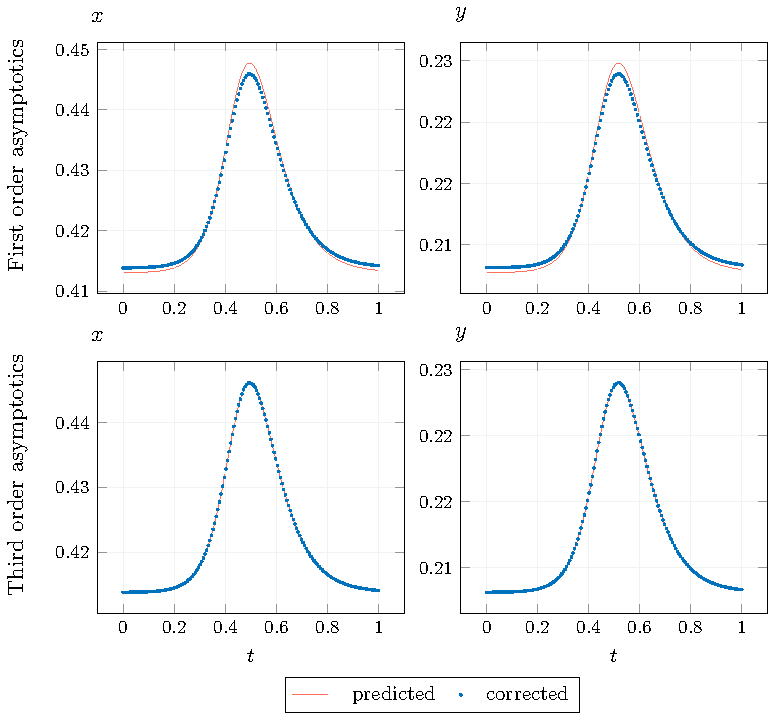
\includegraphics{\imagedir/DoubleAlleeEffectCompareProfiles.pdf}
    \caption{Comparison between the first and third-order asymptotics from
    \cref{btdde:sec:generic_bt_homoclinic_asymptotics} near the generic
        Bogdanov--Takens bifurcation in \cref{sm:eq:double_alle_effect_rescaled} with the
        perturbation parameter set to $\epsilon=0.3$.}
    \label{sm:fig:DoubleAlleeEffectCompareProfiles}
\end{figure}

\subsection{Continuation of the codimension one curves emanating}
To continue the three codimension one curves emanating from the generic
Bogdanov--Takens poin, we can simply use the function
\mintinline[breaklines,breakafter=_]{MATLAB}{C1branch_from_C2point}, as shown in the code below. To monitor the
continuation process, the argument \mintinline{MATLAB}{plot} must be set to \mintinline{MATLAB}{1}.
The most important setting is the perturbation parameter (or multiple),
\mintinline{MATLAB}{step} in the code below. If left out, default step sizes are defined.
However, depending on the problem, no convergence may then be obtained.
\inputminted[firstline=82, lastline=100]{MATLAB}{\pathToDDEBifToolDemos/predator_prey/predator_prey.m}

\subsection{Predictors of the codimension one curves emanating from the Bogdanov--Takens point}
Before we provide the bifurcation diagram in the next section, we first obtain
the predictors for the codimension one curves. For this, we again use the
function \mintinline[breaklines,breakafter=_]{MATLAB}{C1branch_from_C2point}. We set the argument
\mintinline{MATLAB}{predictor} to \mintinline{MATLAB}{1} and provide a range of
perturbation parameters.
\inputminted[firstline=118, lastline=137]{MATLAB}{\pathToDDEBifToolDemos/predator_prey/predator_prey.m}
In the last part of the code above, we added the asymptotics obtained from \cite{Jiao2021}.

\subsection{Bifurcation diagram}
The code below produces a similar figure as \cref{sm:fig:DoubleAlleeEffectCompareParameters} in \MATLAB.
%% Plot the bifurcation curves with predictors
\inputminted[firstline=139, lastline=164]{MATLAB}{\pathToDDEBifToolDemos/predator_prey/predator_prey.m}
%
\begin{figure}[ht]
    \centering
    % this file is generated as a standalone document, to include the reference
    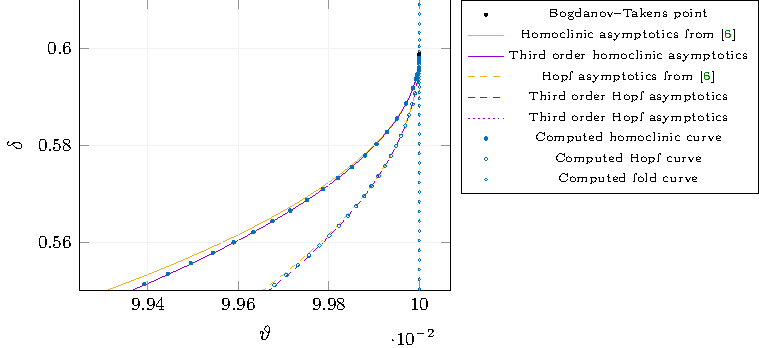
\includegraphics{\imagedir/DoubleAlleeEffectCompareParameters.pdf}
    \caption{Bifurcation diagram near the analytically derived generic Bogdanov-Takens point in
        \cref{sm:eq:double_alle_effect_rescaled} comparing computed codimension one
    curves using \DDEBIFTOOL with the asymptotics obtained in this \paper{} and in \cite{Jiao2021}.}
    \label{sm:fig:DoubleAlleeEffectCompareParameters}
\end{figure}

\subsection{Compare homoclinic solutions in phase-space}
To obtain an impression of the third-order homoclinic asymptotics in
phase-space, we compare the corrected and uncorrected homoclinic solutions
with the perturbation parameter ranging from $0.1$ to $0.3$.
The code below results in \cref{sm:fig:DoubleAlleeEffectCompareOrbitsPhaseSpace}.
We see that the corrected and predicted homoclinic orbits are nearly identical.
\inputminted[firstline=166, lastline=182]{MATLAB}{\pathToDDEBifToolDemos/predator_prey/predator_prey.m}
The \MATLAB console shows the following output.
\begin{minted}{shell-session}
hcli from BT: branch 1 of  1 correction of point 1, success=1
hcli from BT: branch 1 of  1 correction of point 2, success=1
hcli from BT: branch 1 of  1 correction of point 3, success=1
hcli from BT: branch 1 of  1 correction of point 4, success=1
hcli from BT: branch 1 of  1 correction of point 5, success=1
hcli from BT: branch 1 of  1 correction of point 6, success=1
hcli from BT: branch 1 of  1 correction of point 7, success=1
hcli from BT: branch 1 of  1 correction of point 8, success=1
hcli from BT: branch 1 of  1 correction of point 9, success=1
hcli from BT: branch 1 of  1 correction of point 10, success=1
\end{minted}
That is, all predictions in this range are successfully corrected.
%
\begin{figure}[ht]
    \centering
    \includetikzscaled{DoubleAlleeEffectCompareOrbitsPhaseSpace}
    \caption{Plot comparing the third-order homoclinic asymptotics from
    \cref{btdde:sec:generic_bt_homoclinic_asymptotics} near the generic
    Bogdanov--Takens bifurcation in \cref{sm:eq:double_alle_effect_rescaled} with
    the Newton correct homoclinic solutions in $(x,y)$ phase-space.}
    \label{sm:fig:DoubleAlleeEffectCompareOrbitsPhaseSpace}
\end{figure}

\subsection{Convergence plot}
In \cref{sm:fig:DoubleAlleeEffectCompareProfiles} we compared the profiles of
the first and third-order homoclinic asymptotics. Although the improvement of
the third-order asymptotics is clearly visible, a better way to numerically
compare the different orders is by creating a log-log convergence plot. 
Since we create convergence plots for all examples treated in this supplement,
we created the function \mintinline{MATLAB}{convergence_plot}.
\begin{code}
\inputminted{MATLAB}{\pathToDDEBifToolDemos/convergence_plot.m}
\label{sm:lst:convergence_plot}
\caption{Auxiliary function for creating convergence plots.}
\end{code}
Using this function, the code below yields \cref{sm:fig:DoubleAlleeEffectConvergencePlot}.
%% Convergence plot
\inputminted[firstline=184, lastline=195]{MATLAB}{\pathToDDEBifToolDemos/predator_prey/predator_prey.m}
%
\begin{figure}[ht]
    \centering
    \includetikz{DoubleAlleeEffectConvergencePlot}
    \caption{On the abscissa is the approximation to the amplitude $A_0$ and on the ordinate the
        relative error $\delta$ between the constructed solution
        \mintinline{MATLAB}{hcli_pred} to the defining system for the homoclinic orbit and
        the Newton corrected solution \mintinline{MATLAB}{hcli_corrected}.}
    \label{sm:fig:DoubleAlleeEffectConvergencePlot}
\end{figure}



\subsection{Simulation with {\tt DifferentialEquations.jl}}
%
\begin{figure}[ht!]
    \centering
    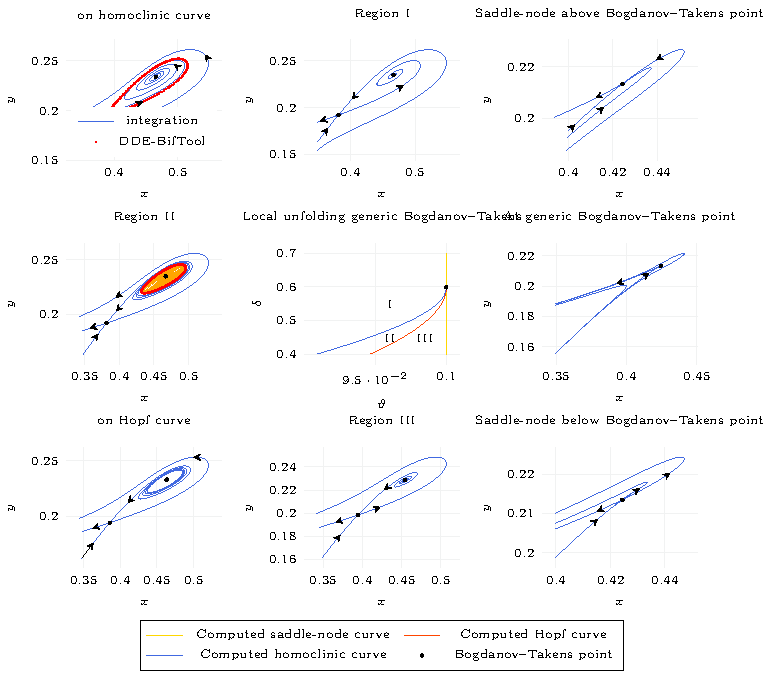
\includegraphics{\imagedir/doubleAlleeEffectSimulation.pdf}
    \caption{Bifurcation diagram near the derived generic Bogdanov-Takens
        point in \cref{sm:eq:neural_network}. In the center, we plotted the
        computed codimension one curves emanating from the Bogdanov--Takens
        point using \DDEBIFTOOL with the third-order homoclinic asymptotics
        obtained in \cref{btdde:sec:generic_bt_homoclinic_asymptotics}. The simulations
        surrounding the center plot have been performed in Julia.}
    \label{sm:fig:double_alle_effect-bifurcation-diagram}
\end{figure}
%
We finish this demonstration by simulating the dynamics near the generic
Bogdanov--Takens point. In \cref{sm:fig:double_alle_effect-bifurcation-diagram}
we created the full local unfolding of the singularity. Note
that, compared with \cite{Jiao2021}, the simulation is done with the original
delay differential equations \cref{sm:eq:double_alle_effect_rescaled} and not
with the ordinary differential equations of the reduced system on the center
manifold. We are able to do this since the parameter-dependent center manifold
is locally attractive. In order to integrate the system in the reverse direction, i.e.,
to obtain the orbits in the stable manifold of the equilibria, we multiplied 
the right-hand size of the system in \cref{sm:eq:double_alle_effect_rescaled} by $-1$.
Note that, in general, this will not provide an accurate approximation at all.
However, since the delay is relatively small, this approximation is accurate
enough for our application. Also, note that the Bogdanov--Takens point still
exists for the approximate system. Nonetheless, even without the backward solutions,
the bifurcation diagram shows that the numerical analysis obtained in
\DDEBIFTOOL is correct.

Since the code for creating the local unfolding diagram is
rather long, we show the code for reproducing the plot simulating the system
near the homoclinic orbit. The code for creating the bifurcation diagram in
\cref{sm:fig:double_alle_effect-bifurcation-diagram} can be found in the
GitHub repository.

\subsubsection{Loading necessary Julia packages}
We start by loading the necessary packages. These are
\begin{itemize}
    \item {\tt DifferentialEquations.jl} A suite for numerically solving differential equations written in Julia.
    \item {\tt GLMakie.jl} For high level plotting on the GPU.
    \item {\tt NonlinearEigenproblems.jl} A nonlinear eigenvalue problem determine a scalar $\lambda$ and a vector $v$ such that $M(\lambda)v=0$. In our case the matrix $M(\lambda)$ will be the characteristic matrix.
    \item {\tt DDEBifTool.jl} We created this very minimalistic package to have some functionality for normal form calculations of DDEs in Julia. Here we use it to calculate the derivatives of the system necessary for {\tt NonlinearEigenproblems.jl}.
    \item {\tt DelimitedFiles.jl} Reading and writing of CSV files.
    \item {\tt PGFPlotsX.jl} A Julia package for creating publication quality figures using the LaTeX library PGFPlots as the backend.
\end{itemize}
\newcommand\pathToJuliaFiles{simulation}
\inputminted[firstline=1, lastline=8]{julia}{\pathToJuliaFiles/predator_prey_simulation_article.jl}

\subsubsection{Define system}
Next we define the system to be integrated, a system to approximate the reverse
flow, and also an allocating version used for stability calculations.
\inputminted[firstline=10, lastline=38]{julia}{\pathToJuliaFiles/predator_prey_simulation_article.jl}

\subsubsection{Functions for plotting arrows} \label{sm:eq:arrow_functions}
We define a function to show in which direction the orbits flow, which is
useful when plotting in phase-space. We also define a function to show the
direction of the leading eigenvectors of the characteristic matrix.

\begin{code}
\inputminted[firstline=40, lastline=71]{julia}{\pathToJuliaFiles/predator_prey_simulation_article.jl}
\caption{Functions for plotting arrows.}
\label{sm:lst:arrow_fucntions}
\end{code}

\subsubsection{Define parameters, equilibria}
We define parameters located on the continued homoclinic branch with
\DDEBIFTOOL. Then define the non-trivial equilibria points in
\cref{sm:eq:double_alle_effect_rescaled}, which can be derived analytically.
\inputminted[firstline=73, lastline=80]{julia}{\pathToJuliaFiles/predator_prey_simulation_article.jl}

\subsubsection{Plot equilibria and homoclinic orbit}
By plotting the homoclinic orbit obtained with \DDEBIFTOOL, we can compare with the numerical simulations. 
\inputminted[firstline=82, lastline=91]{julia}{\pathToJuliaFiles/predator_prey_simulation_article.jl}

\subsubsection{Eigenvectors}
Next, we calculate and plot the leading eigenvectors of the characteristic matrix at the saddle-node bifurcation point.
\inputminted[firstline=93, lastline=105]{julia}{\pathToJuliaFiles/predator_prey_simulation_article.jl}

\subsubsection{Define callback}
Since we are only interested in the flow near the equilibria points, we create a
discrete callback to ensure the orbits do not become too large.
\inputminted[firstline=107, lastline=110]{julia}{\pathToJuliaFiles/predator_prey_simulation_article.jl}

\subsubsection{Integrate the system}
Now we define the problem to be integrated and choose the algorithm to be used.
The first of the five numerical simulations below starts near the unstable
eigendirection. We rotated the eigenvector slightly to follow the homoclinic
orbit very close. The rotation value of $\alpha_0$ was actually obtained by using
the bisection method. However, we did not include this code here. 
\inputminted[firstline=112, lastline=147]{julia}{\pathToJuliaFiles/predator_prey_simulation_article.jl}

\subsubsection{Finish the plot}
Lastly, we add arrows to the obtained solutions using the function
\mintinline{julia}{draw_arrow_on_solution} defined above. Also, we add the
legend and re-plot the equilibria, so that they appear on top.
\inputminted[firstline=149, lastline=161]{julia}{\pathToJuliaFiles/predator_prey_simulation_article.jl}
We should now obtain an interactive figure similar to the left figure in \cref{sm:fig:doubleAlleeEffectHomoclinicSimulation}.
%
\begin{figure}[!ht]
    \centering
    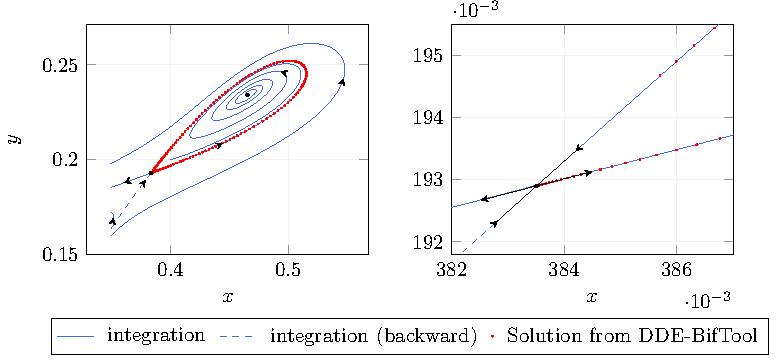
\includegraphics{\imagedir/doubleAlleeEffectHomoclinicSimulation.pdf}
    \caption{Integration of the delayed predator-prey model
        \cref{sm:eq:double_alle_effect_rescaled} at parameter values $(\theta,
        \delta) = (0.094448552842823, 0.447783343351055)$ obtained from
        continuation of the homoclinic curve emanating from the
        Bogdanov--Takens point using \DDEBIFTOOL. In the plot to the right
        a close-up near the saddle is given. Additionally, the 
        leading eigenvectors of the characteristic matrix
        are shown.}
    \label{sm:fig:doubleAlleeEffectHomoclinicSimulation}
\end{figure}


\section[Bogdanov--Takens bifurcation in a neural network model]
        {Generic Bogdanov--Takens bifurcation in a neural network model}

In this example, we will consider the model 
\begin{equation}
\label{sm:eq:neural_network}
\begin{cases}
\mu\dot{u}_1(t) = -u_1(t) + q_{11}\alpha(u_1(t\text{-}T))-q_{12}u_2(t\text{-}T) + e_1,\\
\mu\dot{u}_2(t) = -u_2(t) + q_{21}\alpha(u_1(t\text{-}T))-q_{22}u_2(t\text{-}T) + e_2,
\end{cases}
\end{equation}
which describes the dynamics of a neural network consisting of
excitatory and inhibitory neurons \cite{giannakopoulos2001bifurcations}.
The variables and parameters occurring in \cref{sm:eq:neural_network}
have the following neurophysiological meaning:
\begin{itemize}
\item $u_1,u_2:\mathbb{R}\rightarrow\mathbb{R}$ denote the total post-synaptic
potential of the excitatory and inhibitory neuron, respectively.
\item $\mu>0$ is a time constant characterizing the dynamical properties
of the cell membrane.
\item $q_{ik}\geq0$ represents the strength of the connection line from
the $k$th neuron to the $i$th neuron.
\item $\alpha:\mathbb{R}\rightarrow\mathbb{R}$ is the transfer function
which describes the activity generation of the excitatory neuron as
a function of its total potential $u_1$. The function $\alpha$
is smooth, increasing and has an unique turning point at $u_1 = \theta$.
The transfer function corresponding to the inhibitory neuron is assumed
to be the identity.
\item $T\geq0$ is a time delay reflecting synaptic delay, axonal and dendritic
propagation time.
\item $e_1$ and $e_2$ are external stimuli acting on the excitatory
and inhibitory neuron, respectively.
\end{itemize}

Following \cite{giannakopoulos2001bifurcations}, we consider equation \cref{sm:eq:neural_network} with
\begin{align*}
\alpha(u_1) & = \frac{1}{1 + e^{-4u_1}}-\frac{1}{2},\qquad q_{11} = 2.6,\qquad q_{21} = 1.0,\qquad q_{22} = 0.0,\\
\mu & = 1.0,\qquad T = 1.0,\qquad e_2 = 0.0,
\end{align*}
and $Q: = q_{12},\,E: = e_1$ as bifurcation parameters. Substituting
into \cref{sm:eq:neural_network} yields
\begin{equation}
\label{sm:eq:neural_network_subs}
\begin{cases}
\dot{u}_1(t) = -u_1(t) + 2.6\alpha(u_1(t - 1))-Qu_2(t - 1) + E,\\
\dot{u}_2(t) = -u_2(t) + \alpha(u_1(t - 1)).
\end{cases}
\end{equation}
Notice that for any steady-state we have the symmetry
\begin{equation}
\label{sm:eq:neuralNetworkSymmetry}
    (u_1,u_2,E)\rightarrow(-u_1,-u_2,-E).
\end{equation}
It is easy to explicitly derive that
the system has a double eigenvalue zero for
\begin{equation}
\left\{
\begin{aligned}
    u_1(t) &= \frac14 \log\left(\frac{8 - \sqrt{39}}5\right) \approx -0.2617, \\
    u_2(t) &= -\frac12 \sqrt{\frac{3}{13}} \approx -0.2402, \\
    Q &= \frac{13}{10}, \\
    E &= \frac{\sqrt{39} - 10\atanh \sqrt{\frac{3}{13}}}{20} \approx 0.0505.
\end{aligned}
\right.
\end{equation}

\begin{remark} 
    The \MATLAB files for this demonstration can be found in the directory
    \mintinline[breaklines,breakafter=/]{MATLAB}{demos/tutorial/VII/neural_network_model} relative to the main
    directory of the \DDEBIFTOOL package. Here, we omit the code to generate the
    system file. We assume that the system file
    \mintinline{MATLAB}{sym_neural_network_mf.m} has been
    generated with the script \mintinline{MATLAB}{sym_neural_network.m}. Also, we assume
    that the \DDEBIFTOOL package has been loaded as in
    \cref{sm:lst:searchpath}. The code in
    \crefrange{sm:sec:neural_network_model:pars_and_funcs}{sm:sec:neural_network_model:bifurcation_diagramII}
    highlights the important parts of the file
    \mintinline{MATLAB}{neural_network_model.m}. 
\end{remark}

\subsection{Set parameter names and funcs structure} 
\label{sm:sec:neural_network_model:pars_and_funcs}
As in the previous example, we set the parameter names and define the \mintinline{MATLAB}{funcs} structure.
\inputminted[firstline=28, lastline=39]{MATLAB}{\pathToDDEBifToolDemos/neural_network_model/neural_network_model.m}

\subsection{Set parameter range}
Since we are only interested here in the local unfolding, we restrict the
allowed parameter range for the unfolding parameters. In practice, one may have
physical restrictions which must be satisfied. Additionally, we also limit the
maximum allowed step size during continuation. By doing so, we obtain more refined
data to compare against our predictors.
\inputminted[firstline=41, lastline=44]{MATLAB}{\pathToDDEBifToolDemos/neural_network_model/neural_network_model.m}

\subsection{Stability and coefficients of the generic Bogdanov--Takens point}
We manually construct a steady-state at the generic Bogdanov--Takens point.
\inputminted[firstline=46, lastline=56]{MATLAB}{\pathToDDEBifToolDemos/neural_network_model/neural_network_model.m}
The \MATLAB console shows the following output.
\begin{minted}{shell-session}
ans =

   1.0e-07 *

   0.548156278544666
  -0.548156314155979
\end{minted}
The eigenvalues confirm that the point under consideration is indeed (an
approximation to) a Bogdanov--Takens point. Furthermore, the remaining eigenvalues have
negative real parts. Next, we calculate the normal form coefficients, the
time-reparametrization, and the transformation to the center manifold with the
function \mintinline{MATLAB}{nmfm_bt_orbital}, which implements the coefficients as derived in
\cref{btdde:sec:generic_bogdanov-takens}. For this, we need to set the argument
\mintinline{MATLAB}{free_pars} to the unfolding parameter $(Q,E)$. These
coefficients will be used to start the continuation of the codimension one branches
emanating from the Bogdanov--Takens point.
\inputminted[firstline=58, lastline=62]{MATLAB}{\pathToDDEBifToolDemos/neural_network_model/neural_network_model.m}
The \MATLAB console shows the following output.
\begin{minted}{shell-session}
ans =

  struct with fields:

          a: -0.190382124055415
          b: -0.951910620277072
  theta1000: -0.546026508575597
  theta0001: 1.473611111111115
        K10: [2x1 double]
        K01: [2x1 double]
        K02: [2x1 double]
        K11: [2x1 double]
        K03: [2x1 double]
       phi0: [1x1 struct]
       phi1: [1x1 struct]
      h0010: [1x1 struct]
      h0001: [1x1 struct]
      h2000: [1x1 struct]
      h1100: [1x1 struct]
      h0200: [1x1 struct]
      h1010: [1x1 struct]
      h1001: [1x1 struct]
      h0110: [1x1 struct]
      h0101: [1x1 struct]
      h0002: [1x1 struct]
      h0011: [1x1 struct]
      h3000: [1x1 struct]
      h2100: [1x1 struct]
      h1101: [1x1 struct]
      h2001: [1x1 struct]
      h0003: [1x1 struct]
      h1002: [1x1 struct]
      h0102: [1x1 struct]
          K: @(beta1,beta2)K10*beta1+K01*beta2+1/2*K02*beta2.^2
                +K11*beta1.*beta2+1/6*K03*beta2^3
          H: [function_handle]
\end{minted}
Since the sign of $ab$ is positive, we expect to find unstable periodic orbits nearby the 
Bogdanov--Takens point.

\subsection{Comparing profiles of computed and predicted homoclinic orbits}
To test the homoclinic asymptotics from
\cref{btdde:sec:generic_bt_homoclinic_asymptotics} we compare the first and third
order asymptotics to the Newton corrected solution. For this, we use the 
function \mintinline[breaklines,breakafter=_]{MATLAB}{C1branch_from_C2point}. This function returns a branch, which
by default returns two initial corrected approximations in order to start continuation of the
codimension one curve under consideration. By setting the argument
\mintinline{MATLAB}{'predictor'} to \mintinline{MATLAB}{true} the approximations are left uncorrected.
To make the comparison visually clear, we set the perturbation parameter 
$\epsilon=0.25$ (\mintinline{MATLAB}{step = 0.25} in the code below).
The code below produces \cref{sm:fig:NeuralNetworkCompareProfiles}.
The difference between the two approximations is clearly noticeable. While
the first order asymptotics is close to the Newton corrected solution, the third
order asymptotics is indistinguishable at this scale from the Newton corrected
solution.
\inputminted[firstline=64, lastline=82]{MATLAB}{\pathToDDEBifToolDemos/neural_network_model/neural_network_model.m}
\begin{figure}[ht!]
    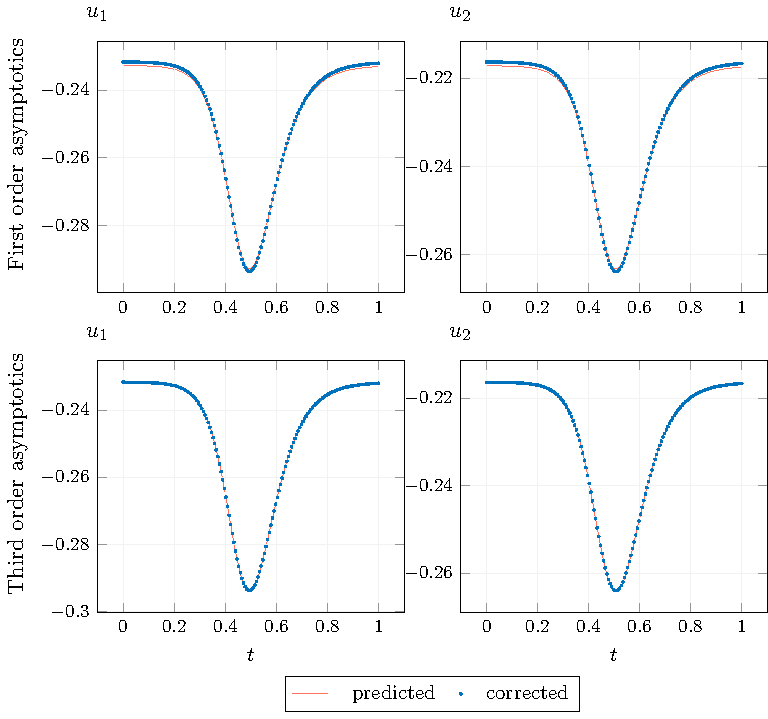
\includegraphics{\imagedir/NeuralNetworkCompareProfiles.pdf}
    \caption{Comparison between the first and third-order asymptotics from
    \cref{btdde:sec:generic_bt_homoclinic_asymptotics} near the generic
        Bogdanov--Takens bifurcation in \cref{sm:eq:neural_network} with the
        perturbation parameter set to $\epsilon=0.25$.}
    \label{sm:fig:NeuralNetworkCompareProfiles}
\end{figure}

\label{sm:sec:neural_network_model:continuation}
\subsection{Continuation of the codimension one curves emanating}
To continue the three codimension one curves emanating from the generic
Bogdanov--Takens point, we can simply use the function
\mintinline[breaklines,breakafter=_]{MATLAB}{C1branch_from_C2point}, as shown in the code below. To monitor the
continuation process, the argument \mintinline{MATLAB}{plot} must be set to \mintinline{MATLAB}{1}.
The most important setting is the perturbation parameter (or multiple),
\mintinline{MATLAB}{step} in the code below. If left out, default step sizes are defined.
However, depending on the problem, no convergence may then be obtained.
\inputminted[firstline=84, lastline=102]{MATLAB}{\pathToDDEBifToolDemos/neural_network_model/neural_network_model.m}

\subsection{Predictors of the codimension one curves emanating from the Bogdanov--Takens point}
Before we provide the bifurcation diagram in the next section, we first obtain the predictors
for the codimension one curves. For this, we again use the function
\mintinline[breaklines,breakafter=_]{MATLAB}{C1branch_from_C2point}. We set the argument \mintinline{MATLAB}{predictor} to \mintinline{MATLAB}{1}
and provide a range of perturbation parameters.
\inputminted[firstline=121, lastline=133]{MATLAB}{\pathToDDEBifToolDemos/neural_network_model/neural_network_model.m}
In the last part of the code above we added the asymptotics obtained from \cite{Jiao2021}.

\subsection{Bifurcation diagram}
The code below produces (a figure similar to) \cref{sm:fig:NeuralNetworkCompareParameters}.
%% Plot the bifurcation curves with predictors
\inputminted[firstline=135, lastline=156]{MATLAB}{\pathToDDEBifToolDemos/neural_network_model/neural_network_model.m}
%
\begin{figure}[ht]
    \centering
    \includetikzscaled{NeuralNetworkCompareParameters}
    \caption{Bifurcation diagram near the derived generic Bogdanov-Takens point in
        \cref{sm:eq:neural_network} comparing computed codimension one curves using
        \DDEBIFTOOL with the third-order homoclinic parameter asymptotics obtained
        in \cref{btdde:sec:generic_bt_homoclinic_asymptotics}.}
    \label{sm:fig:NeuralNetworkCompareParameters}
\end{figure}

\subsection{Compare homoclinic solutions in phase-space}
To obtain an impression of the third-order homoclinic asymptotics in
phase-space, we compare the corrected and uncorrected homoclinic solutions
with the perturbation parameter ranging from $0.1$ to $0.3$.
The code below results in \cref{sm:fig:NeuralNetworkCompareOrbitsPhaseSpace}.
We see that the corrected and predicted homoclinic orbits are nearly identical.
\inputminted[firstline=158, lastline=174]{MATLAB}{\pathToDDEBifToolDemos/neural_network_model/neural_network_model.m}
%
\begin{figure}[ht]
    \centering
    \includetikzscaled{NeuralNetworkCompareOrbitsPhaseSpace}
    \caption{Plot comparing the third-order homoclinic asymptotics from
        \cref{btdde:sec:generic_bt_homoclinic_asymptotics} near the generic
        Bogdanov--Takens bifurcation in \cref{sm:eq:neural_network} with the
        Newton correct homoclinic solutions in $(u_1,u_2)$ phase-space.}
    \label{sm:fig:NeuralNetworkCompareOrbitsPhaseSpace}
\end{figure}

\subsection{Convergence plot}
Using the function from \cref{sm:lst:convergence_plot}, we create a log-log
convergence plot comparing the convergence order of the first and thrid order
homoclinic asymptotics from \cref{btdde:sec:generic_bt_homoclinic_asymptotics}.
The code below yields \cref{sm:fig:NeuralNetworkConvergencePlot}.
\inputminted[firstline=176, lastline=187]{MATLAB}{\pathToDDEBifToolDemos/neural_network_model/neural_network_model.m}
\begin{figure}[ht]
    \centering
    \includetikz{NeuralNetworkConvergencePlot}
        \caption{On the abscissa is the approximation to the amplitude $A_0$ and on
        the ordinate the relative error $\delta$ between the constructed solution
        \mintinline{MATLAB}{hcli_pred} to the defining system for the homoclinic orbit
        and the Newton corrected solution \mintinline{MATLAB}{hcli_corrected}.}
    \label{sm:fig:NeuralNetworkConvergencePlot}
\end{figure}

\subsection{Continuation of the codimension one curves emanating from the second Bogdanov--Takens point}
For completeness, we also continue the codimension one curves emanating from
the second Bogdanov--Takens point, which exists due to the symmetry
\cref{sm:eq:neuralNetworkSymmetry}. Of course, we could just use the symmetry
instead of computing the curves numerically. However, we use it as an
additional verification of our derived asymptotics. The code below defines the
second Bogdanov--Takens point, calculates the stability, and continues the Hopf
and homoclinic bifurcation curves.
\inputminted[firstline=189, lastline=216]{MATLAB}{\pathToDDEBifToolDemos/neural_network_model/neural_network_model.m}

\subsection{Bifurcation diagram with two Bogdanov--Takens points}
\label{sm:sec:neural_network_model:bifurcation_diagramII}
Now that we continued the Hopf and homoclinic bifurcation curves emanating from
the second Bogdanov--Takens point, we can reconstruct the bifurcation diagram
given in \cite[Figure 7]{giannakopoulos2001bifurcations}. The code below
results into a similar figure as \cref{sm:fig:NeuralNetworkCompareParametersII} in \MATLAB.
\inputminted[firstline=218, lastline=245]{MATLAB}{\pathToDDEBifToolDemos/neural_network_model/neural_network_model.m}
\begin{figure}[ht]
    \centering
    \includetikzscaled{NeuralNetworkCompareParametersII}
    \caption{Reconstruction of the bifurcation diagram given in \cite[Figure
        7]{giannakopoulos2001bifurcations}. We could have used the symmetry
        \cref{sm:eq:neuralNetworkSymmetry} instead of computing the additional
        curves numerically. However, it provides us an additional verification of
        our derived asymptotics.}
    \label{sm:fig:NeuralNetworkCompareParametersII}
\end{figure}

\subsection{Simulation with {\tt DifferentialEquations.jl}}
Here we will perform two simulations. The first simulation will be at the
double homoclinic orbits, which will confirm the continuation of both
homoclinic orbits and is also ascetically pleasing, see \cref{sm:fig:NeuralNetworkSimulationHomoclinic}. The second simulation will
be in the region where there should be unstable periodic orbits, see \cref{sm:fig:NeuralNetworkPeriodicSimulation}.

\begin{figure}[ht]
    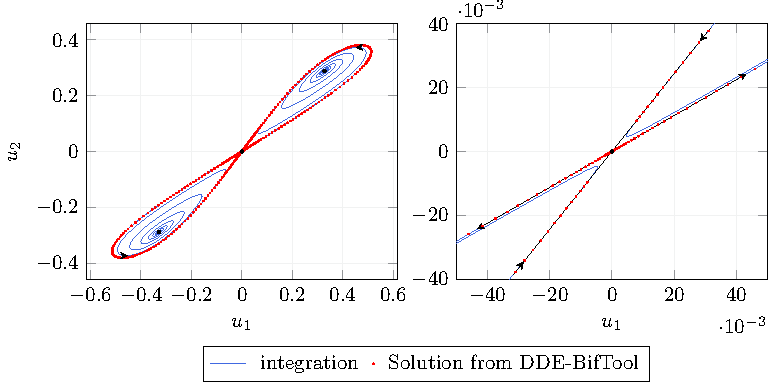
\includegraphics{\imagedir/NeuralNetworkDoubleHomoclinicSimulation.pdf}
    \caption{Comparing the computed double homoclinic orbit in \cref{sm:eq:neural_network}
    with \DDEBIFTOOL with the solutions obtained from numerical simulation with Julia.
    In the right plot is a close-up near the equilibrium at the origin. Also, the
    leading stable and unstable eigenvectors of the characteristic matrix are plotted. We see the numerical integrated solution
    intersects all the red points from the solution from \DDEBIFTOOL.}
    \label{sm:fig:NeuralNetworkSimulationHomoclinic}
\end{figure}

\begin{figure}[ht]
    \centering
    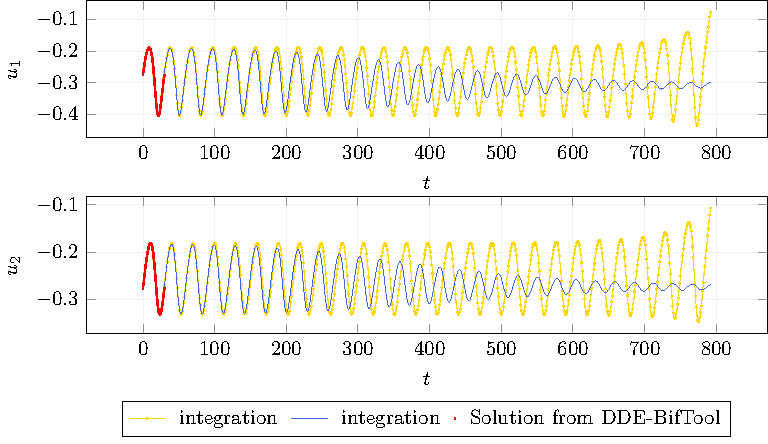
\includegraphics{\imagedir/NeuralNetworkPeriodicSimulation.pdf}
    \caption{Comparing a computed periodic orbit in \cref{sm:eq:neural_network}
        with \DDEBIFTOOL at $(Q,E)=(1.476442865781454, 0.0)$ with the solution
        obtained from numerical simulation with Julia near the periodic orbit.
        The yellow dotted line has the constant history function $(u_1,u_2) =
        (-0.274863341578762, -0.27715979849863204)$ slightly below the periodic
        orbit.  The blue line has the constant history function $(u_1,u_2) =
        (-0.274863341578762, -0.276969798498632)$, a point on the periodic
        orbit (red dots) located with \DDEBIFTOOL.
    }
    \label{sm:fig:NeuralNetworkPeriodicSimulation}
\end{figure}

\subsubsection{Loading necessary Julia packages}
We start by loading the necessary packages.

%
\begin{listing}[h!!]
\inputminted[firstline=1, lastline=6]{julia}{\pathToJuliaFiles/neural_network_model_simulation_article.jl}
\caption{Loading Julia packages for simulation in \cref{sm:eq:neural_network}.}
\label{sm:lst:neuralNetworkLoadingPacakges}
\end{listing}

In the previous demonstration we were able to derive the equilibria
analytically.  Here we will solve for the equilibria numerically with the
packages {\tt IntervalArithmetic.jl} \cite{IntervalArithmetic} and  {\tt
IntervalRootFinding.jl} \cite{IntervalRootFinding}.

\subsubsection{Define system}
We define the system to be integrated, a system to approximate the reverse
flow, and also an allocating version used for stability calculations.
\inputminted[firstline=8, lastline=27]{julia}{\pathToJuliaFiles/neural_network_model_simulation_article.jl}

\subsubsection{Functions for plotting arrows}
We define a function to show in which direction the orbits flow, which is
useful when plotting in phase-space. We also define functions to show the
direction of the leading eigenvectors of the characteristic matrix.
The code is shown in \cref{sm:lst:arrow_fucntions}.

\subsubsection{Create figure with several axes}
We create a figure containing multiple axis in which we will plot the bifurcation diagram and
the homoclinic and periodic orbits.
\inputminted[firstline=63, lastline=73]{julia}{\pathToJuliaFiles/neural_network_model_simulation_article.jl}

\subsubsection{Plot bifurcation diagram in the middle}
Loading the continued bifurcation curves obtained with \DDEBIFTOOL and plot these in the middle axis.
This should give a similar bifurcation diagram as in \cref{sm:fig:NeuralNetworkCompareParametersII}.
\inputminted[firstline=76, lastline=102]{julia}{\pathToJuliaFiles/neural_network_model_simulation_article.jl}

\subsubsection{Simulation at the double homoclinic orbit}
In the code below we integrate at parameter values $(Q,E)=(1.459868437376222,0)$, i.e.,
where we located the double homoclinic orbit. We start by locating the three equilibria
points. Note that by the symmetry we actually only need to solve for one of them.
We calculate the stability of the equilibria and filter out the leading stable and unstable
eigenvectors from the characteristic matrix of the saddle-node point. 
The rest of the code should be pretty straight forward,
since it is very similar as in the simulation in the previous demonstration.
After running this code, we should obtain a similar plot as in
the left plot of \cref{sm:fig:NeuralNetworkSimulationHomoclinic}.
\inputminted[firstline=105, lastline=166]{julia}{\pathToJuliaFiles/neural_network_model_simulation_article.jl}

\subsubsection{Simulation near an unstable periodic orbit}
To show by integration the existence of an unstable periodic orbit, we first
located a periodic orbit in \DDEBIFTOOL. This can be done by continuing a
branch of periodic orbits emanating from a point on the continued Hopf curve.
Then we load the profiles of the periodic orbits into Julia and start
integration near the perioidic orbits.  After running the code below, we should
obtain a similar plot as in
\cref{sm:fig:NeuralNetworkPeriodicSimulation}.
\inputminted[firstline=169, lastline=208]{julia}{\pathToJuliaFiles/neural_network_model_simulation_article.jl}




\section[the Van der Pol oscillator with delay feedback]
        {Transcritical Bogdanov--Takens bifurcation in the Van der Pol oscillator with delay feedback}
We consider the Van der Pol oscillator with delay feedback \cite{jiang2007bogdanov}
given by 
\begin{equation}
\ddot{x}(t) + \epsilon(x^2(t)-1)\dot{x}(t) + x(t) = \epsilon g(x(t-\tau))\label{sm:eq:dde_vanderPol}
\end{equation}
where $\epsilon>0$ is a parameter, $\tau>0$ is a delay and $g:\mathbb{R}\rightarrow\mathbb{R}$
is a smooth function with $g(0) = 0$ and $g'(0)\neq0$. We rewrite
the Van der Pol equation \cref{sm:eq:dde_vanderPol} as
\begin{equation}
\label{sm:eq:vanderPolOscillator}
\begin{cases}
    \dot{x}_1 = x_2,\\
    \dot{x}_2 = \epsilon g(x_1(t-\tau))-\epsilon(x_1^2-1)x_2-x_1.
\end{cases}
\end{equation}
Rescaling time with $t\rightarrow\dfrac{t}{\tau}$ to normalize the
delay yields
\begin{equation}
\label{sm:eq:vanderPolOscillatorRescaled}
\begin{cases}
\dot{x}_1 = \tau x_2,\\
\dot{x}_2 = \tau\left(\epsilon g(x_1(t-1))-\epsilon(x_1^2-1)x_2-x_1\right).
\end{cases}
\end{equation}
This allows to treat $\tau$ as a bifurcation parameter.

Following \cite{jiang2007bogdanov}, we consider \cref{sm:eq:dde_vanderPol} with
\[
g(x) = \frac{e^x-1}{c_1e^x + c_2},
\]
where $c_1 = \dfrac{1}{4}$ and $c_2 = \dfrac{1}{2}$. Then the trivial
equilibrium undergoes a transcritical Bogdanov--Takens bifurcation at parameter
values $(\epsilon,\tau) = (0.75,0.75)$, \cite{jiang2007bogdanov} and the
supplement. 

\begin{remark}
    The \MATLAB files for this demonstration can be found in the directory
    \mintinline[breaklines,breakafter=/]{MATLAB}{demos/tutorial/VII/vdpo_bt_transcritical} relative to the main
    directory of the \DDEBIFTOOL package. Here, we omit the code to generate a
    system file. The system file \mintinline{MATLAB}{sym_vdpo_mf.m} has been generated
    with the script \mintinline{MATLAB}{sym_vdpo_mf.m}. Also, we assume that the
    \DDEBIFTOOL package has been loaded as in \cref{sm:lst:searchpath}. The
    code in
    \crefrange{sm:sec:vpdo:pars_and_funcs}{sm:sec:vdpo:convergence_plot}
    highlights the important parts of the file
    \mintinline{MATLAB}{vanderPolOscillator.m}. 
\end{remark}

\subsection{Set parameter names and funcs structure}
\label{sm:sec:vpdo:pars_and_funcs}
As in the previous example, we set the parameter names and define the \mintinline{MATLAB}{funcs} structure.
\inputminted[firstline=31, lastline=37]{MATLAB}{\pathToDDEBifToolDemos/vdpo_bt_transcritical/vanderPolOscillator.m}

\subsection{Set parameter range}
Since we are only interested here in the local unfolding, we restrict the
allowed parameter range for the unfolding parameters. In practice, one may have
physical restrictions which must be satisfied. Additionally, we also limit the
maximum allowed step size during continuation. By doing so, we obtain more refined
data to compare against our predictors.
\inputminted[firstline=39, lastline=42]{MATLAB}{\pathToDDEBifToolDemos/vdpo_bt_transcritical/vanderPolOscillator.m}

\subsection{Stability and coefficients of the transcritical Bogdanov--Takens point}
We manually construct a steady-state at the transcritical Bogdanov--Takens
point and calculate its stability.
\inputminted[firstline=44, lastline=55]{MATLAB}{\pathToDDEBifToolDemos/vdpo_bt_transcritical/vanderPolOscillator.m}

The \MATLAB console shows the following output.
\begin{minted}{shell-session}
ans =

   1.0e-07 *

       0.6223
      -0.6223

\end{minted}
The eigenvalues confirm that the point under consideration is indeed (an
approximation to) a Bogdanov--Takens point. Furthermore, the remaining eigenvalues have
negative real parts. Next, we calculate the normal form coefficients, the
time-reparametrization, and the transformation to the center manifold with the
function \mintinline{MATLAB}{nmfm_bt_orbital}, which implements the coefficients as derived in
\cref{btdde:sec:transcritical-Bogdanov-Takens}. For this, we need to set the argument
\mintinline{MATLAB}{free_pars} to the unfolding parameter $(Q,E)$. These
coefficients will be used to start the continuation of the codimension one branches
emanating from the Bogdanov--Takens point. Also, since we are in the transcritical case,
we set the argument \mintinline{matlab}{generic_unfolding} to \mintinline{matlab}{false}.
\inputminted[firstline=57, lastline=60]{MATLAB}{\pathToDDEBifToolDemos/vdpo_bt_transcritical/vanderPolOscillator.m}

The \MATLAB console shows the following output.
\begin{minted}{shell-session}
ans =

  struct with fields:

          a: 0.1304
          b: -0.2949
  theta1000: 0.0780
  theta0010: -21.1293
  theta0001: -0.3811
       phi0: [1x1 struct]
       phi1: [1x1 struct]
      h2000: [1x1 struct]
      h1100: [1x1 struct]
      h0200: [1x1 struct]
      h3000: [1x1 struct]
      h2100: [1x1 struct]
        K10: [2x1 double]
        K01: [2x1 double]
        K02: [2x1 double]
        K11: [2x1 double]
        K20: [2x1 double]
      h1010: [1x1 struct]
      h1001: [1x1 struct]
      h0110: [1x1 struct]
      h0101: [1x1 struct]
      h2010: [1x1 struct]
      h1110: [1x1 struct]
      h2001: [1x1 struct]
      h1101: [1x1 struct]
      h1002: [1x1 struct]
      h0102: [1x1 struct]
      h1020: [1x1 struct]
      h0120: [1x1 struct]
      h1011: [1x1 struct]
      h0111: [1x1 struct]
          K: @(beta1,beta2)K10*beta1+K01*beta2+1/2*K20*beta1^2
                    +K11*beta1*beta2+1/2*K02*beta2^2
          H: [function_handle]
\end{minted}
Since the sign of $ab$ is negative, we expect to find stable periodic orbits nearby the 
Bogdanov--Takens point.

\subsection{Comparing profiles of computed and predicted homoclinic orbits}
To test the homoclinic asymptotics from
\cref{btdde:sec:generic_bt_homoclinic_asymptotics} we compare the first and third
order asymptotics to the Newton corrected solution. For this, we use the 
function \mintinline[breaklines,breakafter=_]{MATLAB}{C1branch_from_C2point}. This function returns a branch, which
by default returns two initial corrected approximations in order to start continuation of the
codimension one curve under consideration. By setting the argument
\mintinline{MATLAB}{'predictor'} to \mintinline{MATLAB}{true} the approximations are left uncorrected.
To make the comparison visually clear, we set the perturbation parameter 
$\epsilon=0.1$ (\mintinline{MATLAB}{step = 0.1} in the code below).
The code below produces \cref{sm:fig:VDPOCompareProfiles}.
The difference between the two approximations is clearly noticeable. While
the first order asymptotics is close to the Newton corrected solution, the third
order asymptotics is indistinguishable at this scale from the Newton corrected
solution.
\inputminted[firstline=63, lastline=87]{MATLAB}{\pathToDDEBifToolDemos/vdpo_bt_transcritical/vanderPolOscillator.m}

\begin{figure}[ht]
    \centering
    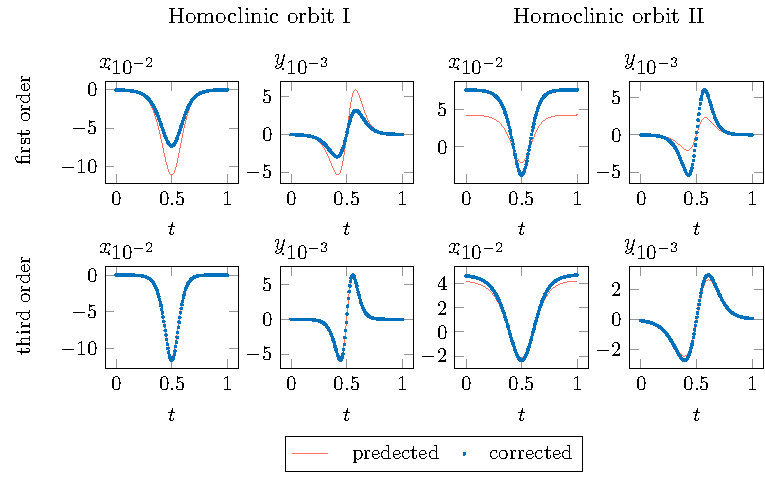
\includegraphics{\imagedir/VDPOCompareProfiles.pdf}
    \caption{Comparison between the first and third-order homoclinic asymptotics from
    \cref{btdde:sec:transcritical_bt_homoclinic_asymptotics} near the transcritical
        Bogdanov--Takens bifurcation in \cref{sm:eq:vanderPolOscillatorRescaled} with the
        perturbation parameter set to $\epsilon=0.1$.}
    \label{sm:fig:VDPOCompareProfiles}
\end{figure}

\subsection{Continuation of the codimension one curves emanating}
To continue the three codimension one curves emanating from the generic
Bogdanov--Takens point, we can simply use the function
\mintinline[breaklines,breakafter=_]{MATLAB}{C1branch_from_C2point}, as shown in the code below. To monitor the
continuation process, the argument \mintinline{MATLAB}{plot} must be set to \mintinline{MATLAB}{1}.
The most important setting is the perturbation parameter (or multiple),
\mintinline{MATLAB}{step} in the code below. If left out, default step sizes are defined.
However, depending on the problem, no convergence may then be obtained.
\inputminted[firstline=89, lastline=113]{MATLAB}{\pathToDDEBifToolDemos/vdpo_bt_transcritical/vanderPolOscillator.m}

\subsection{Predictors of the codimension one curves emanating from the Bogdanov--Takens point}
Before we provide the bifurcation diagram in the next section, we first obtain the predictors
for the codimension one curves. For this, we again use the function
\mintinline[breaklines,breakafter=_]{MATLAB}{C1branch_from_C2point}. We set the argument \mintinline{MATLAB}{predictor} to \mintinline{MATLAB}{1}
and provide a range of perturbation parameters.
\inputminted[firstline=135, lastline=154]{MATLAB}{\pathToDDEBifToolDemos/vdpo_bt_transcritical/vanderPolOscillator.m}

\subsection{Bifurcation diagram}
The code below produces (a figure similar to) \cref{sm:fig:DoubleAlleeEffectCompareParameters}.
\inputminted[firstline=156, lastline=182]{MATLAB}{\pathToDDEBifToolDemos/vdpo_bt_transcritical/vanderPolOscillator.m}
%
\begin{figure}[ht]
    \centering
    \includetikzscaled{vanderPolOscillatorCompareParameters}
    \caption{Bifurcation diagram near the derived transcritical Bogdanov-Takens point in
        \cref{sm:eq:vanderPolOscillatorRescaled} comparing computed codimension one curves using
        \DDEBIFTOOL with the third-order homoclinic parameter asymptotics obtained
        in \cref{btdde:sec:transcritical_bt_homoclinic_asymptotics}.}
    \label{sm:fig:VDPOCompareParameters}
\end{figure}

\subsection{Compare homoclinic solutions in phase-space}
To obtain an impression of the third-order homoclinic asymptotics in
phase-space, we compare the corrected and uncorrected homoclinic solutions
with the perturbation parameter ranging from $0.01$ to $0.03$.
The code below produces (a figure similar to) \cref{sm:fig:VDPOCompareOrbitsPhaseSpace}.
We see that the corrected and predicted homoclinic orbits are nearly identical.
\inputminted[firstline=203, lastline=230]{MATLAB}{\pathToDDEBifToolDemos/vdpo_bt_transcritical/vanderPolOscillator.m}
%
\begin{figure}[ht!]
    \centering
    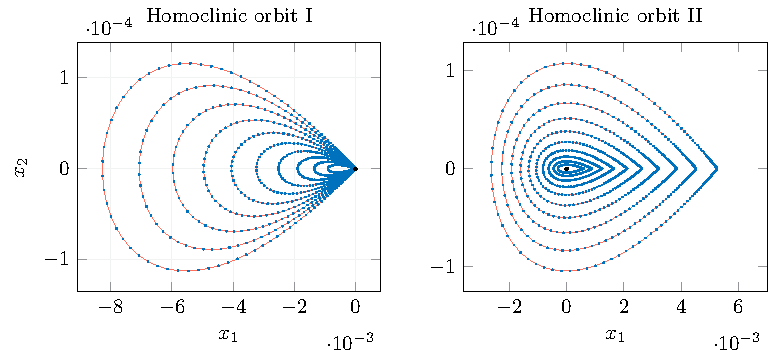
\includegraphics{\imagedir/VDPOCompareOrbitsPhaseSpace.pdf} \\
    \vspace*{20pt}
    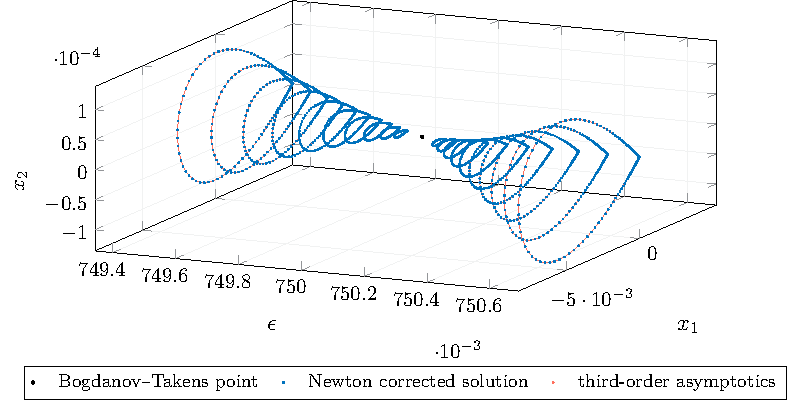
\includegraphics{\imagedir/VDPOCompareOrbitsPhaseSpaceBottom.pdf}
    \caption{Plot comparing the third-order homoclinic asymptotics from
        \cref{btdde:sec:transcritical_bt_homoclinic_asymptotics} near the
        transcritical Bogdanov--Taken in
        \cref{sm:eq:vanderPolOscillatorRescaled} with the Newton correct
        homoclinic solutions phase-space with the perturbation parameter
        $\epsilon$ ranging from $0.01$ to $0.03$.}
    \label{sm:fig:VDPOCompareOrbitsPhaseSpace}
\end{figure}

\subsection{Convergence plot}
\label{sm:sec:vdpo:convergence_plot}
Using the function from \cref{sm:lst:convergence_plot}, we create a log-log
convergence plot comparing the convergence order of the first and thrid order
homoclinic asymptotics from \cref{btdde:sec:transcritical_bt_homoclinic_asymptotics}.
The code below yields \cref{sm:fig:VDPOConvergencePlot}.
\inputminted[firstline=232, lastline=243]{MATLAB}{\pathToDDEBifToolDemos/vdpo_bt_transcritical/vanderPolOscillator.m}
%
\begin{figure}[ht]
    \centering
    \includetikz{VDPOConvergencePlot}
        \caption{On the abscissa is the approximation to the amplitude $A_0$ and on
        the ordinate the relative error $\delta$ between the constructed solution
        \mintinline{MATLAB}{hcli_pred} to the defining system for the homoclinic orbit
        and the Newton corrected solution \mintinline{MATLAB}{hcli_corrected}.}
    \label{sm:fig:VDPOConvergencePlot}
\end{figure}

\subsection{Simulation with {\tt DifferentialEquations.jl}}
Here we will perform four simulations. The first two simulations will be at two
homoclinic orbits located on the two homoclinic curves emanating from the
transcritical Bogdanov--Takens point continued with \DDEBIFTOOL, see
\cref{sm:fig:VDPOSimulationHomoclinic}. The second two simulations will be in
the regions where there should be stable periodic orbits, see
\cref{sm:fig:VDPOPeriodicSimulation}.

\begin{figure}[ht]
    \centering
    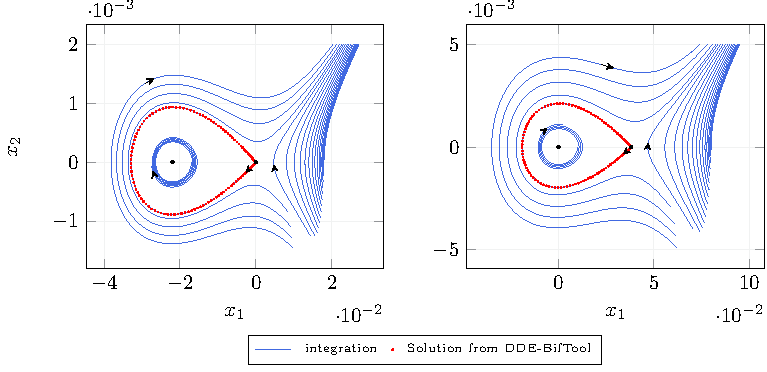
\includegraphics{\imagedir/VDPOHomoclinicSimulation.pdf}
    \caption{Comparing the computed homoclinic orbits in \cref{sm:eq:vanderPolOscillatorRescaled}
    with \DDEBIFTOOL with the solutions obtained from numerical simulation with Julia.
    We see the numerical integrated solution
    going through all the red points from the solution from \DDEBIFTOOL.}
    \label{sm:fig:VDPOSimulationHomoclinic}
\end{figure}

\begin{figure}[ht]
    \centering
    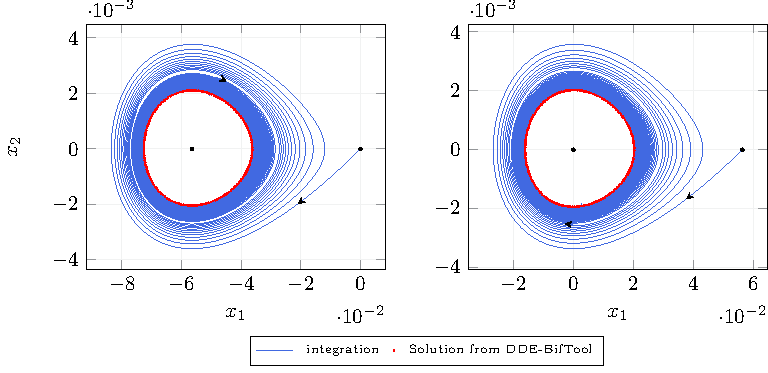
\includegraphics{\imagedir/VDPOPeriodicSimulation.pdf}
    \caption{Comparing the computed periodic orbits in \cref{sm:eq:vanderPolOscillatorRescaled}
    with \DDEBIFTOOL with the solutions obtained from numerical simulation with Julia.
    We see the numerical integrated solution
    going through all the red points from the solution from \DDEBIFTOOL.}
    \label{sm:fig:VDPOPeriodicSimulation}
\end{figure}

\subsubsection{Loading necessary Julia packages}
Since we do not have  analytical expressions for the equilibria, we load the
same Julia packges as in the previous demonstration, see
\cref{sm:lst:neuralNetworkLoadingPacakges}.

\subsubsection{Define system}
We define the system to be integrated and also an allocating version used for
stability calculations.
\inputminted[firstline=8, lastline=30]{julia}{\pathToJuliaFiles/vdpo_simulation_article.jl}

\subsubsection{Functions for plotting arrows}
We define a function to show in which direction the orbits flow, which is
useful when plotting in phase-space. We also define functions to show the
direction of the leading eigenvectors of the characteristic matrix.
The code is shown in \cref{sm:lst:arrow_fucntions}.

\subsubsection{Function for creating streamlines plot}
To obtain an impression of the flow near transcritical Bogdanov--Takens point,
we create a streamlines function. This is particularly useful for seeing the
flow around the stable manifold of the saddle-note.
\inputminted[firstline=65, lastline=77]{julia}{\pathToJuliaFiles/vdpo_simulation_article.jl}

\subsubsection{Create figure with several axes}
We create a figure containing multiple axis in which we will plot 
the two homoclinic and two periodic orbits.
\inputminted[firstline=79, lastline=84]{julia}{\pathToJuliaFiles/vdpo_simulation_article.jl}

\subsubsection{Define parameters, equilibria}
We define parameters located on the continued homoclinic branch with
\DDEBIFTOOL. Then calculate the equilibria points in
\cref{sm:eq:vanderPolOscillatorRescaled} near the transcritical
Bogdanov--Takens point.
\inputminted[firstline=86, lastline=93]{julia}{\pathToJuliaFiles/vdpo_simulation_article.jl}

\subsubsection{Plot equilibria and homoclinic orbit}
By plotting the homoclinic orbit obtained with \DDEBIFTOOL located at parameter
values 
\[
    (\epsilon_0, \tau_0) = (0.752774810893411, 0.754736729675371),
\]
we can compare with the numerical simulations.
\inputminted[firstline=95, lastline=101]{julia}{\pathToJuliaFiles/vdpo_simulation_article.jl}

\subsubsection{Leading eigenvectors}
Next, we calculate and plot the leading eigenvectors of the characteristic matrix at the saddle-node bifurcation point.
\inputminted[firstline=103, lastline=117]{julia}{\pathToJuliaFiles/vdpo_simulation_article.jl}

\subsubsection{Define callback}
Since we are only interested in the flow near the equilibria points, we create a
discrete callback to ensure the orbits do not become too large.
\inputminted[firstline=122, lastline=125]{julia}{\pathToJuliaFiles/vdpo_simulation_article.jl}

\subsubsection{Integrate the system at homoclinic orbits I}
Now we define the problem to be integrated and choose the algorithm to be used.
Then we integrate the system for a range of initial history functions using the
function \mintinline{julia}{streamlines}. Next, we integrate the system near
the inner equillibrium, i.e., the equilbrium inside the homoclinic orbit. This
equilibria should be an unstable spiral. By using the unstable eigenvector of the
characteristic matrix, we obtain a solution going through the homoclinic solution
obtained with \DDEBIFTOOL.
\inputminted[firstline=127, lastline=152]{julia}{\pathToJuliaFiles/vdpo_simulation_article.jl}

\subsubsection{Add arrows on solutions}
Lastly, we add arrows to the obtained solutions using the function
\mintinline{julia}{draw_arrow_on_solution} defined above.
\inputminted[firstline=154, lastline=158]{julia}{\pathToJuliaFiles/vdpo_simulation_article.jl}
We should now obtain an interactive figure similar to the left figure in \cref{sm:fig:VDPOSimulationHomoclinic}.

\subsubsection{Simulation near stable periodic orbit I}
The code for numerical simulation near the second homoclinic orbit, see the
right plot in \cref{sm:fig:VDPOSimulationHomoclinic}, is almost identical to
the code above for the first homoclinic orbit and is therefore not included
here.

To show by integration the existence of an stable periodic orbit, we first
located a periodic orbit in \DDEBIFTOOL. This can be done by continuing a
branch of periodic orbits emanating from a point on the continued Hopf curves.
Then we load the profiles of the periodic orbits into Julia. We perform two
simulations. For the first simulation, we integrate with a constant history
function equal to a point inside the periodic orbit. The second starts from the
unstable eigenvector of the characteristic matrix calculated above.
\inputminted[firstline=230, lastline=279]{julia}{\pathToJuliaFiles/vdpo_simulation_article.jl}
After running the above code, we should obtain a similar plot as in \cref{sm:fig:VDPOPeriodicSimulation}.
\begin{remark}
By the intersection of the orbits in the first simulation, we see that, although
the system on the center manifold is equivalent to an ODE, the system we
integrate is still a DDE.
\end{remark}


\section[Tri-neuron BAM neural network model]
        {Transcritical Bogdanov--Takens bifurcation in a tri-neuron BAM neural network model}
We consider a three-component system of a tri-neuron bidirectional
associative memory (BAM) neural network model with multiple delays
\cite{dong2013bogdanov}. The architecture of this BAM model is illustrated in
\cref{sm:fig:BAM_architecture_graph}. 

\begin{figure}
\centering
\includetikzscaled[0.75]{BAM_architecture_graph}
\caption{The graph of architecture for model \cref{sm:eq:tri_neuron_BAM}}
\label{sm:fig:BAM_architecture_graph}
\end{figure}

In this model, there is only one neuron with the activation function
$f_{1}$ on the $I$-layer and there are two neurons with respective
activation functions $f_{2}$ and $f_{3}$ on the $J$-layer. We assume
that the time delay from the $I$-layer to the $J$-layer is $\tau_{1}$,
while the time delay from the $J$-layer to the $I$-layer is $\tau_{2}$.
Then the network can be described by the following delay differential equation:
\begin{equation}
\label{sm:eq:tri_neuron_BAM}
\begin{aligned}
\begin{cases}
\dot{x}_{1}(t) = -\mu_{1}x_{1}(t)+c_{21}f_{1}(x_{2}(t-\tau_{2}))+c_{31}f_{1}(x_{3}(t-\tau_{2})),\\
\dot{x}_{2}(t) = -\mu_{2}x_{2}(t)+c_{12}f_{2}(x_{1}(t-\tau_{1})),\\
\dot{x}_{3}(t) = -\mu_{3}x_{3}(t)+c_{13}f_{3}(x_{1}(t-\tau_{1})),
\end{cases}
\end{aligned}
\end{equation}
where:
\begin{itemize}
\item $x_{i}(t)\,(i=1,2,3)$ denote the state of the neuron at time $t$;
\item $\mu_{i}(i=1,2,3)$ describe the attenuation rate of internal neurons
processing on the $I$-layer and the $J$-layer and $\mu_{i}>0$;
\item the real constants $c_{i1}$and $c_{1i}\,(2,3)$ denote the neurons
in two layers: the $I$-layer and the $J$-layer.
\end{itemize}
Letting $u_{1}(t)=x_{1}(t-\tau_{1}),u_{2}(t)=x_{2}(t),u_{3}(t)=x_{3}(t)$
and $\tau=\tau_{1}+\tau_{2}$, then system \cref{sm:eq:tri_neuron_BAM}
is equivalent to the following system:

\begin{equation}
\label{sm:eq:tri_neuron_BAM-u}
\begin{cases}
\dot{u}_{1}(t) = -\mu_{1}u_{1}(t)+c_{21}f_{1}(u_{2}(t-\tau))+c_{31}f_{1}(u_{3}(t-\tau)),\\
\dot{u}_{2}(t) = -\mu_{2}u_{2}(t)+c_{12}f_{2}(u_{1}(t)),\\
\dot{u}_{3}(t) = -\mu_{3}u_{3}(t)+c_{13}f_{3}(u_{1}(t)).
\end{cases}
\end{equation}

\begin{lemma}
\label{sm:lem:BAM_double_eigenvalue}
Assume that $f_{i}(0)=0\,(i=1,2,3)$, $f_{i}'(0)\neq0\,(i=1,2,3)$ and
$\mu_{2}\neq\mu_{3}$, then the steady-state $(u_{1},u_{2},u_{3})=(0,0,0)$ has a
double zero eigenvalue at 
\begin{align*}
c_{21} & =c_{21}^{0}=\frac{\mu_{2}^{2}\left(\mu_{1}\left(\mu_{3}\tau+1\right)+\mu_{3}\right)}{c_{12}\left(\mu_{2}-\mu_{3}\right)f_{1}'(0)f_{2}'(0)},\\
c_{31} & =c_{31}^{0}=\frac{\mu_{3}^{2}\left(\mu_{1}\left(\mu_{2}\tau+1\right)+\mu_{2}\right)}{c_{13}\left(\mu_{3}-\mu_{2}\right)f_{1}'(0)f_{3}'(0)}.
\end{align*}
\end{lemma}
\begin{proof}
The characteristic matrix of \cref{sm:eq:tri_neuron_BAM-u} is given
by
\[
\Delta(\lambda)=\left(\begin{array}{ccc}
\lambda+\mu_{1} & -e^{-\lambda\tau}c_{21}f_{1}'(0) & -e^{-\lambda\tau}c_{31}f_{1}'(0)\\
-c_{12}f_{2}'(0) & \lambda+\mu_{2} & 0\\
-c_{13}f_{3}'(0) & 0 & \lambda+\mu_{3}

\end{array}\right).
\]
Thus, the characteristic equation becomes 
\begin{align}
\det\Delta(\lambda) & =\lambda^{3}+\left(\mu_{1}+\mu_{2}+\mu_{3}\right)\lambda^{2}+\big(-c_{12}c_{21}f_{1}'(0)f_{2}'(0)e^{-\lambda\tau}\nonumber \\
 & \qquad-c_{13}c_{31}f_{1}'(0)f_{3}'(0)e^{-\lambda\tau}+\mu_{1}\mu_{2}+\mu_{3}\mu_{2}+\mu_{1}\mu_{3}\big)\lambda\nonumber \\
 & \qquad+\mu_{1}\mu_{2}\mu_{3}-e^{-\lambda\tau}\left(c_{12}c_{21}\mu_{3}f_{2}'(0)+c_{13}c_{31}\mu_{2}f_{3}'(0)\right)f_{1}'(0)=0.\label{sm:eq:BAM_characteristic_eq}
\end{align}

Clearly, $\lambda=0$ is a root if and only if
\[
\mu_{1}\mu_{2}\mu_{3}=\left(c_{12}c_{21}\mu_{3}f_{2}'(0)+c_{13}c_{31}\mu_{2}f_{3}'(0)\right)f_{1}'(0).
\]
Taking the derivative of \cref{sm:eq:BAM_characteristic_eq} with respect
to $\lambda$ gives
\begin{align}
\dfrac{d}{d\lambda}\det\Delta(\lambda) & =3\lambda^{2}+2\left(\mu_{1}+\mu_{2}+\mu_{3}\right)\lambda+\big(-c_{12}c_{21}f_{1}'(0)f_{2}'(0)e^{-\lambda\tau}\nonumber \\
 & \qquad-c_{13}c_{31}f_{1}'(0)f_{3}'(0)e^{-\lambda\tau}+\mu_{1}\mu_{2}+\mu_{3}\mu_{2}+\mu_{1}\mu_{3}\big)\nonumber \\
 & \qquad+\tau\left(c_{12}c_{21}f_{2}'(0)e^{-\lambda\tau}+c_{13}c_{31}f_{3}'(0)e^{-\lambda\tau}\right)f_{1}'(0)\lambda\nonumber \\
 & \qquad+\tau e^{-\lambda\tau}\left(c_{12}c_{21}\mu_{3}f_{2}'(0)+c_{13}c_{31}\mu_{2}f_{3}'(0)\right)f_{1}'(0)=0.\label{sm:eq:BAM_characteristic_eq-derivative}
\end{align}
Therefore, we have
\begin{align*}
    \det\Delta'(0) &= \big(-c_{12}c_{21}f_{1}'(0)f_{2}'(0)-c_{13}c_{31}f_{1}'(0)f_{3}'(0)+\mu_{1}\mu_{2}+\mu_{3}\mu_{2}+\mu_{1}\mu_{3}\big)=0.
\end{align*}

For any $\tau>0$, it is easy to see that $\det\Delta(\lambda)=\det\Delta'(\lambda)=0$,
if and only if the following conditions are satisfied
\begin{equation}
\begin{cases}
\left((1-\tau\mu_{3})c_{12}c_{21}f_{2}'(0)+(1-\tau\mu_{2})c_{13}c_{31}f_{3}'(0)\right)f_{1}'(0)=\mu_{1}\mu_{2}+\mu_{3}\mu_{2}+\mu_{1}\mu_{3},\\
\\
\left(c_{12}c_{21}\mu_{3}f_{2}'(0)+c_{13}c_{31}\mu_{2}f_{3}'(0)\right)f_{1}'(0)=\mu_{1}\mu_{2}\mu_{3}.
\end{cases}\label{sm:eq:BAM_double_eigvalue_zero_condition}
\end{equation}
By solving \cref{sm:eq:BAM_double_eigvalue_zero_condition} for $(c_{21},c_{31})$
we get $(c_{21},c_{31})=(c_{21}^{0},c_{31}^{0})$.
Taking the derivative of \cref{sm:eq:BAM_characteristic_eq-derivative}
yields
\begin{align}
\dfrac{d^{2}}{d\lambda^{2}}\det\Delta(\lambda) & =6\lambda+2\left(\mu_{1}+\mu_{2}+\mu_{3}\right)+\tau f_{1}'(0)\big(c_{12}c_{21}f_{2}'(0)e^{-\lambda\tau}+c_{13}c_{31}f_{3}'(0)e^{-\lambda\tau}\big)\nonumber \\
 & \qquad+\tau\left(c_{12}c_{21}f_{2}'(0)e^{-\lambda\tau}+c_{13}c_{31}f_{3}'(0)e^{-\lambda\tau}\right)f_{1}'(0)\nonumber \\
 & \qquad-\tau^{2}\left(c_{12}c_{21}f_{2}'(0)e^{-\lambda\tau}+c_{13}c_{31}f_{3}'(0)e^{-\lambda\tau}\right)f_{1}'(0)\lambda\nonumber \\
 & \qquad-\tau^{2}e^{-\lambda\tau}\left(c_{12}c_{21}\mu_{3}f_{2}'(0)+c_{13}c_{31}\mu_{2}f_{3}'(0)\right)f_{1}'(0)=0.\label{sm:eq:BAM_characteristic_eq-derivative-1}
\end{align}
Then we can obtain
\begin{align*}
 & \dfrac{d^{2}}{d\lambda^{2}}\det\Delta(0)\vert_{(c_{21},c_{31})=(c_{21}^{0},c_{31}^{0})}\\
 & \quad=2\left(\mu_{1}+\mu_{2}+\mu_{3}\right)+2\tau f_{1}'(0)\big(c_{12}c_{21}^{0}f_{2}'(0)+c_{13}c_{31}^{0}f_{3}'(0)\big)\\
 & \qquad-\tau^{2}f_{1}'(0)\left(c_{12}c_{21}^{0}\mu_{3}f_{2}'(0)+c_{13}c_{31}^{0}\mu_{2}f_{3}'(0)\right)\\
 & \quad=2\left(\mu_{1}+\mu_{2}+\mu_{3}\right)+\tau\left(\frac{\mu_{2}^{2}\left(\mu_{1}\left(\mu_{3}\tau+1\right)+\mu_{3}\right)}{\left(\mu_{2}-\mu_{3}\right)}+\frac{\mu_{3}^{2}\left(\mu_{1}\left(\mu_{2}\tau+1\right)+\mu_{2}\right)}{\left(\mu_{3}-\mu_{2}\right)}\right)\\
 & \qquad-\tau^{2}\left(\frac{\mu_{2}^{2}\left(\mu_{1}\left(\mu_{3}\tau+1\right)+\mu_{3}\right)}{\left(\mu_{2}-\mu_{3}\right)}\mu_{3}+\frac{\mu_{3}^{2}\left(\mu_{1}\left(\mu_{2}\tau+1\right)+\mu_{2}\right)}{\left(\mu_{3}-\mu_{2}\right)}\mu_{2}\right)\\
 & \quad=2\left(\mu_{1}+\mu_{2}+\mu_{3}\right)+2\tau\left(\mu_{1}\mu_{2}+\mu_{1}\mu_{3}+\mu_{2}\mu_{3}\right)+\tau^{2}\mu_{1}\mu_{2}\mu_{3}.
\end{align*}

Since $\tau>0$ and $\mu_{i}>0 (i=1,2,3)$ the second derivative of
the characteristic equations at $(\lambda,c_{21},c_{31})=(0,c_{21}^{0},c_{31}^{0})$
does not vanish, and we obtain a double zero eigenvalue.
\end{proof}

\begin{lemma}
\label{sm:lemma:triNeuralBAMNetworkModelEigenvalues}
\textup{Correction to \cite[Lemma 3]{dong2013bogdanov}}
Let $(c_{21},c_{31})=(c_{21}^{0},c_{31}^{0})$,
\begin{equation}
    \label{sm:eq:triNeuralBAMNetworkModel:omega_0} 
    \omega_0 = \frac{\sqrt{-\mu_1^2 - \mu_2^2 - \mu_3^2 + \sqrt{\zeta_0}}}{\sqrt{2}}
\end{equation}
and $0<\tau<\tau_{0}$, where $\tau_0$ is the minimum positive solution to the nonlinear equation
\begin{equation}
    \label{sm:eq:triNeuralBAMNetworkModel:tan} 
    \tan (\tau \omega_0) = \frac{b_0\zeta_1 - a_0\zeta_2}{a_0\zeta_1 + b_0\zeta_2},
\end{equation}
with
\begin{align*}
a_0 &= -\mu_1\mu_2\mu_3, \\ 
b_0 &= -\omega_0(\mu_2\mu_3 + \mu_1(\mu_2 + \mu_3 + \mu_2\mu_3\tau)), \\
\zeta_0 &= \mu_1^4 + (\mu_2^2 + \mu_3^2)^2 + 8\mu_1\mu_2\mu_3(\mu_2 + \mu_3 + \mu_2\mu_3\tau) + \\
        &\qquad 2\mu_1^2(\mu_3^2 + 4\mu_2\mu_3(1 + \mu_3\tau) + \mu_2^2(1 + 2\mu_3\tau(2 + \mu_3\tau))), \\
\zeta_1 &= \mu_1\mu_2\mu_3 - (\mu_1 + \mu_2 + \mu_3)\omega_0^2, \\
\zeta_2 &= \mu_2\mu_3\omega_0 + \mu_1(\mu_2 + \mu_3)\omega_0 - \omega_0^3.
\end{align*}
Then all roots of the characteristic equation \cref{sm:eq:BAM_characteristic_eq},
except the double zero roots, have negative real parts.
\end{lemma}

\begin{proof}
Consider that there are eigenvalues $\lambda\neq0$ on the imaginary
axis for $(c_{21}^{0},c_{31}^{0})$. Substituting $\lambda=i\omega,(\omega>0)$
and $(c_{21}^{0},c_{31}^{0})$ into \cref{sm:eq:BAM_characteristic_eq},
and rearranging terms according to its real and imaginary part yields
\begin{equation}
\label{sm:eq:BAM_real_imag_parts_char_eq}
-\begin{pmatrix}
    \zeta_1 \\
    \zeta_2 
\end{pmatrix}
=
\begin{pmatrix}
    a_0 & \phantom{-}b_0 \\
    b_0 & -a_0
\end{pmatrix}
\begin{pmatrix}
\cos\tau\omega \\
\sin\tau\omega
\end{pmatrix}.
\end{equation}
By squaring and adding the above equations, it follows that
\begin{equation}
    \label{sm:eq:BAM_omega}
    \zeta_1^2 + \zeta_2^2 = a_0^2 + b_0^2.
\end{equation}
Solving the equation for positive $\omega>0$ yields \cref{sm:eq:triNeuralBAMNetworkModel:omega_0}.

Next, from \cref{sm:eq:BAM_real_imag_parts_char_eq}, we obtain \cref{sm:eq:triNeuralBAMNetworkModel:tan}.
First notice that $\tau \mapsto \omega_0 \tau$ is a strictly increasing
function since it is the product of two strictly increasing positive functions.
It follows that $\tau \mapsto \tan \omega_0 \tau$ is periodic in $\tau$ with
range $\mathbb R$. The next observation is that the denominator in the right-hand
side of \cref{sm:eq:triNeuralBAMNetworkModel:tan} has a unique positive root $\tau=\tau_1$, at which
that numerator does not vanish. In fact, it can be checked that the numerator
does never vanish. Lastly, taking the limit of the right-hand side of
\cref{sm:eq:triNeuralBAMNetworkModel:tan} of $\tau$ to infinity is $0$, i.e.
\[
    \lim_{\tau \rightarrow \infty} \frac{-b_0\zeta_1 + a_0\zeta_2}{\phantom{-}a_0\zeta_1 + b_0\zeta_2} = 0.
\]
By the continuity of the right-hand side, it follows that \cref{sm:eq:triNeuralBAMNetworkModel:tan} has
countable many solutions in $\tau$. Let $\tau_0$ be the minimum positive 
solution. Since for $\tau=0$ all solutions to the characteristic equation, except
of the double zero eigenvalue at the origin, have negative real parts.
We conclude by \cite[Corollary 2.3]{Ruan@2001} that
all eigenvalues, except for the double zero eigenvalues, are located
in the left half plane for $0 < \tau < \tau_0$.
\end{proof}

\begin{remark}
    Note that, although $(\omega,\tau) = (\omega_0,\tau_0)$, solves \cref{sm:eq:triNeuralBAMNetworkModel:tan,sm:eq:BAM_omega},
    this not necessary means it solves the original equations \cref{sm:eq:BAM_real_imag_parts_char_eq}.
    Thus, the center manifold may still be stable for values $\tau>\tau_0$. We will demonstrate this
    in the example below.
\end{remark}

For the numerical verification we consider, as in the simulations in
\cite[Example 1]{dong2013bogdanov}, the system \cref{sm:eq:tri_neuron_BAM-u} with
the activation functions
\begin{equation}
    \label{sm:eq:triNeuralBAMNetworkModelFunctions}
    f_{1}(x)=\tanh(x)+0.1x^{2},\quad f_{2}(x)=f_{3}(x)=\tanh(x),
\end{equation}
and parameter values
\begin{equation}
    \label{sm:eq:triNeuralBAMNetworkModelFixedParameters}
    \mu_{1}=0.1,\mu_{2}=0.3,\mu_{3}=0.2,c_{12}=c_{13}=1,\tau=5.
\end{equation}
Then, from \cref{sm:lem:BAM_double_eigenvalue}, we obtain two critical
values 
\[
(c_{21}^{0},c_{31}^{0})=(0.36,-0.22),
\]
at which there is a transcritical Bogdanov--Takens point. Furthermore, since
$\tau < \tau_0 \approx 5.4320$ the center manifold is locally attractive. In
fact, we will show below that the center manifold is locally attractive for
$0<\tau<13.2309348879375$.

\begin{remark}
    The \MATLAB files for this demonstration can be found in the directory
    \mintinline[breaklines,breakafter=/]{MATLAB}{demos/tutorial/VII/BAM_neural_network_model} relative to the main
    directory of the package \DDEBIFTOOL. Here, we omit the code to generate a
    system file. The system file\\
    \mintinline{MATLAB}{sym_BAMnn_mf.m} has been
    generated with the script \mintinline{MATLAB}{sym_BAMnn.m}. Also, we assume
    that the \DDEBIFTOOL package has been loaded as in
    \cref{sm:lst:searchpath}. The code in
    \crefrange{sm:sec:tri_neuron_BAM:pars_and_funcs}
              {sm:sec:tri_neuron_BAM:convergence_plot}
    highlights the important parts of the file
    \mintinline{MATLAB}{BAMnn.m}. 
\end{remark}

\subsection{Set parameter names and funcs structure} 
\label{sm:sec:tri_neuron_BAM:pars_and_funcs}
As in the previous example, we set the parameter names and define the \mintinline{MATLAB}{funcs} structure.
\inputminted[firstline=27, lastline=33]{MATLAB}{\pathToDDEBifToolDemos/BAM_neural_network_model/BAMnn.m}


\subsection{Set parameter range}
Since we are only interested here in the local unfolding, we restrict the
allowed parameter range for the unfolding parameters. In practice, one may have
physical restrictions which must be satisfied. Additionally, we also limit the
maximum allowed step size during continuation. By doing so, we obtain more refined
data to compare against our predictors.
\inputminted[firstline=35, lastline=38]{MATLAB}{\pathToDDEBifToolDemos/BAM_neural_network_model/BAMnn.m}

\subsection{Stability and coefficients of the transcritical Bogdanov--Takens point}
We manually construct a steady-state at the transcritical Bogdanov--Takens
point and calculate its stability.
\inputminted[firstline=40, lastline=49]{MATLAB}{\pathToDDEBifToolDemos/BAM_neural_network_model/BAMnn.m}

The \MATLAB console shows the following output.
\begin{minted}{shell-session}
ans =

  -0.0000 + 0.0000i
  -0.0000 - 0.0000i
  -0.2246 + 0.6600i
  -0.2246 - 0.6600i
  -0.6371 + 1.8063i
  -0.6371 - 1.8063i
  -0.8483 + 3.0681i
  -0.8483 - 3.0681i
  -0.9849 + 4.3336i
  -0.9849 - 4.3336i
\end{minted}
The eigenvalues confirm that the point under consideration is indeed (an
approximation to) a Bogdanov--Takens point. Furthermore, the remaining eigenvalues have
negative real parts. Next, we calculate the normal form coefficients, the
time-reparametrization, and the transformation to the center manifold with the
function \mintinline{MATLAB}{nmfm_bt_orbital}, which implements the coefficients as derived in
\cref{btdde:sec:transcritical-Bogdanov-Takens}. For this, we need to set the argument
\mintinline{MATLAB}{free_pars} to the unfolding parameter $(\alpha_1,\alpha_2)$. These
coefficients will be used to start the continuation of the codimension one branches
emanating from the Bogdanov--Takens point. Also, since we are in the transcritical case,
we set the argument \mintinline{matlab}{generic_unfolding} to \mintinline{matlab}{false}.
\inputminted[firstline=51, lastline=55]{MATLAB}{\pathToDDEBifToolDemos/BAM_neural_network_model/BAMnn.m}

The \MATLAB console shows the following output.
\begin{minted}{shell-session}

ans =

  struct with fields:

          a: 0.0012
          b: -0.0135
  theta1000: -2.5813
  theta0010: 3.1322e+03
  theta0001: -190.0753
       phi0: [1x1 struct]
       phi1: [1x1 struct]
      h2000: [1x1 struct]
      h1100: [1x1 struct]
      h0200: [1x1 struct]
      h3000: [1x1 struct]
      h2100: [1x1 struct]
        K10: [2x1 double]
        K01: [2x1 double]
        K02: [2x1 double]
        K11: [2x1 double]
        K20: [2x1 double]
      h1010: [1x1 struct]
      h1001: [1x1 struct]
      h0110: [1x1 struct]
      h0101: [1x1 struct]
      h2010: [1x1 struct]
      h1110: [1x1 struct]
      h2001: [1x1 struct]
      h1101: [1x1 struct]
      h1002: [1x1 struct]
      h0102: [1x1 struct]
      h1020: [1x1 struct]
      h0120: [1x1 struct]
      h1011: [1x1 struct]
      h0111: [1x1 struct]
          K: @(beta1,beta2)K10*beta1+K01*beta2+1/2*K20*beta1^2
                    +K11*beta1*beta2+1/2*K02*beta2^2
          H: [function_handle]

\end{minted}
Since the sign of $ab$ is negative, we expect to find stable periodic orbits nearby the 
Bogdanov--Takens point.

\subsection{Comparing profiles of computed and predicted homoclinic orbits}
To test the homoclinic asymptotics from
\cref{btdde:sec:generic_bt_homoclinic_asymptotics} we compare the first and third
order asymptotics to the Newton corrected solution. For this, we use the 
function \mintinline[breaklines,breakafter=_]{MATLAB}{C1branch_from_C2point}. This function returns a branch, which
by default returns two initial corrected approximations in order to start continuation of the
codimension one curve under consideration. By setting the argument
\mintinline{MATLAB}{'predictor'} to \mintinline{MATLAB}{true} the approximations are left uncorrected.
To make the comparison visually clear, we set the perturbation parameter 
$\epsilon=0.02$ (\mintinline{MATLAB}{step = 0.02} in the code below).
The code below produces \cref{sm:fig:TriNeuronBAMCompareProfilesI,sm:fig:TriNeuronBAMCompareProfilesII}.
The difference between the two approximations is clearly noticeable. While
the first order asymptotics is close to the Newton corrected solution, the third
order asymptotics is indistinguishable at this scale from the Newton corrected
solution.
\inputminted[firstline=57, lastline=81]{MATLAB}{\pathToDDEBifToolDemos/BAM_neural_network_model/BAMnn.m}

\begin{figure}[ht]
    \centering
    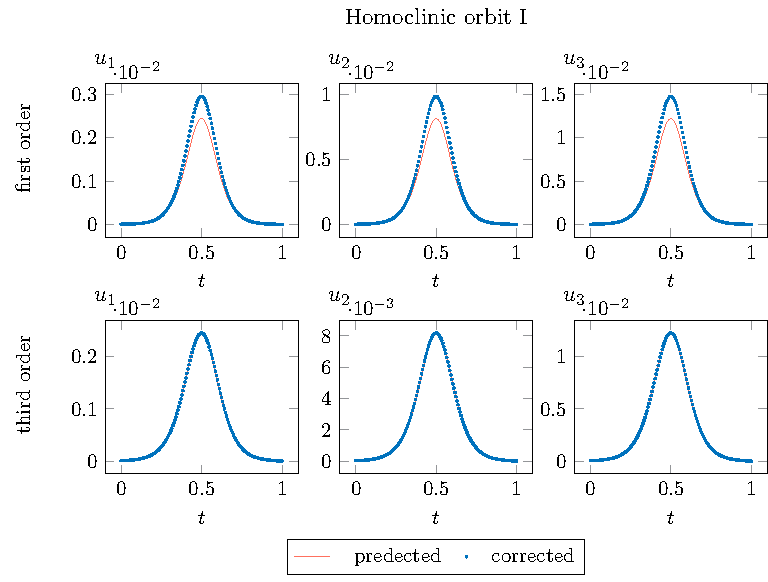
\includegraphics{\imagedir/TriNeuronBAMCompareProfilesI.pdf}
    \caption{Comparison between the first and third-order homoclinic asymptotics from
    \cref{btdde:sec:transcritical_bt_homoclinic_asymptotics} near the transcritical
        Bogdanov--Takens bifurcation in \cref{sm:eq:tri_neuron_BAM} with the
        perturbation parameter set to $\epsilon=0.02$.}
        \label{sm:fig:TriNeuronBAMCompareProfilesI}
\end{figure}

\begin{figure}[ht]
    \centering
    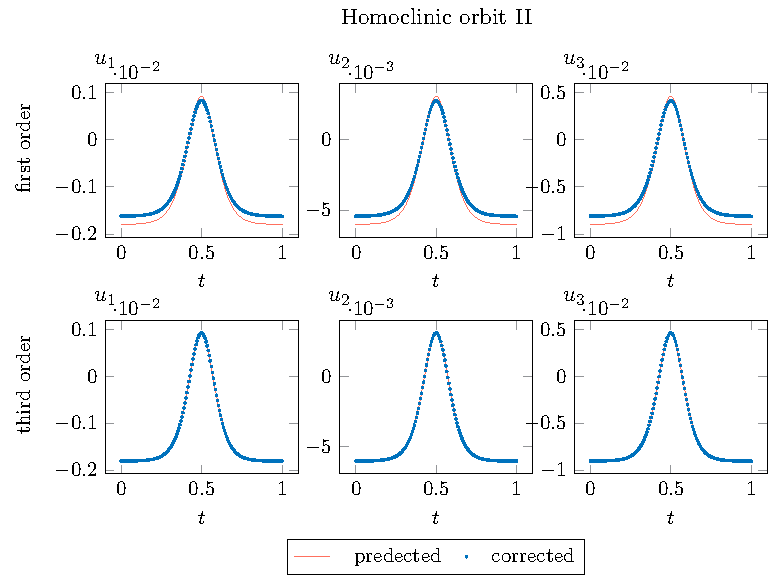
\includegraphics{\imagedir/TriNeuronBAMCompareProfilesII.pdf}
    \caption{Comparison between the first and third-order homoclinic asymptotics from
    \cref{btdde:sec:transcritical_bt_homoclinic_asymptotics} near the transcritical
        Bogdanov--Takens bifurcation in \cref{sm:eq:tri_neuron_BAM} with the
        perturbation parameter set to $\epsilon=0.02$.}
        \label{sm:fig:TriNeuronBAMCompareProfilesII}
\end{figure}

\subsection{Continuation of the codimension one curves emanating}
To continue the three codimension one curves emanating from the generic
Bogdanov--Takens point, we can simply use the function
\mintinline{MATLAB}{C1branch_from_C2point}, as shown in the code below. To monitor the
continuation process, the argument \mintinline{MATLAB}{plot} must be set to \mintinline{MATLAB}{1}.
The most important setting is the perturbation parameter (or multiple),
\mintinline{MATLAB}{step} in the code below. If left out, default step sizes are defined.
However, depending on the problem, no convergence may then be obtained.
\inputminted[firstline=83, lastline=103]{MATLAB}{\pathToDDEBifToolDemos/BAM_neural_network_model/BAMnn.m}

\subsection{Predictors of the codimension one curves emanating from the Bogdanov--Takens point}
Before we provide the bifurcation diagram in the next section, we first obtain the predictors
for the codimension one curves. For this, we again use the function
\mintinline{MATLAB}{C1branch_from_C2point}. We set the argument \mintinline{MATLAB}{predictor} to \mintinline{MATLAB}{1}
and provide a range of perturbation parameters.
\inputminted[firstline=127, lastline=146]{MATLAB}{\pathToDDEBifToolDemos/BAM_neural_network_model/BAMnn.m}

\subsection{Bifurcation diagram}
The code below produces (a figure similar to) \cref{sm:fig:triNeuronBAMNeuralNetworkModelCompareParametersSupplementI}.
\inputminted[firstline=148, lastline=175]{MATLAB}{\pathToDDEBifToolDemos/BAM_neural_network_model/BAMnn.m}
%
\begin{figure}[ht]
\includetikzscaled{triNeuronBAMNeuralNetworkModelCompareParametersSupplementI}
\caption{Bifurcation diagram near the analytically derived transcritical
    Bogdanov--Takens point in \cref{sm:eq:tri_neuron_BAM} comparing the
    computed codimension one curves emanating form the Bogdanov--Takens point
    using \DDEBIFTOOL with the third-order homoclinic parameter asymptotics
    obtained in \cref{btdde:sec:transcritical_bt_homoclinic_asymptotics}.}
\label{sm:fig:triNeuronBAMNeuralNetworkModelCompareParametersSupplementI}
\end{figure}

\subsection{Detect bifurcations on the second Hopf branch}
We can use the \DDEBIFTOOL function \mintinline{MATLAB}{LocateSpecialPoints} to
locate bifurcation points on the second Hopf banch.
\inputminted[firstline=177, lastline=178]{MATLAB}{\pathToDDEBifToolDemos/BAM_neural_network_model/BAMnn.m}

Inspecting the \MATLAB output gives.
\begin{minted}{shell-session}
HopfCodimension2: calculate stability if not yet present
HopfCodimension2: calculate L1 coefficients
HopfCodimension2: (provisional) 2 gen. Hopf 2 Takens-Bogdanov  detected.
br_insert: detected 1 of 4: genh. Normalform:
    L2: 5.7933e+03
    L1: 1.0106e-09

br_insert: detected 2 of 4: BT. Normalform:
    a2: -5.8499e-04
    b2: -0.0031

br_insert: detected 3 of 4: genh. Normalform:
    L2: -5.7933e+03
    L1: -2.1214e-09

br_insert: detected 4 of 4: BT. Normalform:
    a2: -0.0012
    b2: 0.0135
\end{minted}
Thus, there are two Bogdanov--Takens points detected. By inspection of the normal
form coefficients $a$ and $b$ (\mintinline{MATLAB}{a2} and
\mintinline{MATLAB}{b2} in the output above) with the coefficients of the
transcritical Bogdanov--Takens point, we see that one is (very likely) already
known. Indeed, while continuing the second Hopf curve from the transcritical
Bogdanov--Takens point, we encounter another Bogdanov--Takens point, at which
the Hopf curve turns around, and continues in the reverse direction, back to
the transcritical Bogdanov--Takens point. Similarly, we also deduce that there
is only one generalized Hopf point detected on the Hopf curve. Inspecting 
the parameters indeed confirm our claim.

Since the newly detected Bogdanov--Takens point is on the Hopf curve
on which the equilibrium changes position under variation of the
parameters, we extract the Bogdanov--Takens point and computed the coefficients
of the generic case.
\inputminted[firstline=179, lastline=181]{MATLAB}{\pathToDDEBifToolDemos/BAM_neural_network_model/BAMnn.m}

\subsection{Plot Bogdanov-Takens test function along the Hopf curve}
Before we continu the homoclinic branch emanating from the generic
Bogdanov--Takens point, we first plot the testfunction for the Bogdanov--Takens
point, i.e. we plot the imaginary part for the critical eigenvalues along the
second Hopf curve. The code below produces (a figure similar to)
\cref{sm:fig:triNeuronBAMNeuralNetworkModelTestfunction}.
\inputminted[firstline=185, lastline=197]{MATLAB}{\pathToDDEBifToolDemos/BAM_neural_network_model/BAMnn.m}
%
\begin{figure}[ht]
    \centering
    \includetikzscaled{triNeuronBAMNeuralNetworkModelTestfunction}
    \caption{Plot of the Bogdanov--Takens testfunction along the second Hopf curve. 
    We see that surface $\omega=0$ is intersected transversally two times
    while continuing the Hopf curve.}
    \label{sm:fig:triNeuronBAMNeuralNetworkModelTestfunction}
\end{figure}

\subsection{Continue third homoclinic curve}
The code below continuous the homoclinic solution emanating from the generic Bogdanov--Takens detected
on the second Hopf branch. The last line extracts the parameters used for plotting.
\inputminted[firstline=199, lastline=205]{MATLAB}{\pathToDDEBifToolDemos/BAM_neural_network_model/BAMnn.m}

\subsection{Bifurcation plot}
We are now in the position to recreate the bifurcation plot as shown in the main text. There, we
left out the predictors for the codimension one equilibria bifurcation curves and changed the color
of the computed codimension one equilibria curves to gray. In this way focus will be on
the homoclinic curves. The code below produces (a figure similar to)
\cref{sm:fig:triNeuronBAMNeuralNetworkModelCompareParameters}.
\inputminted[firstline=213, lastline=243]{MATLAB}{\pathToDDEBifToolDemos/BAM_neural_network_model/BAMnn.m}
\begin{figure}[ht]
    \includetikzscaled{triNeuronBAMNeuralNetworkModelCompareParameters}
    \caption{
    Bifurcation diagram near the transcritical and generic Bogdanov--Takens
    bifurcation points in \cref{sm:eq:tri_neuron_BAM-u} comparing computed
    codimension one curves using \DDEBIFTOOL with the asymptotics obtained in the 
    main text.}
    \label{sm:fig:triNeuronBAMNeuralNetworkModelCompareParameters}
\end{figure}

\subsection{Large view bifurcation plot without predictors}
Although the first and third homoclinic bifurcation curves exist only in a very small
parameter region, the second is continued in a relatively large parameter range. The
code below produces (a figure similar to)
\cref{sm:fig:triNeuronBAMNeuralNetworkModelLargerBifurctionPlot}.
\inputminted[firstline=245, lastline=267]{MATLAB}{\pathToDDEBifToolDemos/BAM_neural_network_model/BAMnn.m}
\begin{figure}[ht]
    \includetikzscaled{triNeuronBAMNeuralNetworkModelLargerBifurctionPlot}
    \caption{
    Bifurcation diagram near the transcritical and
    a generic Bogdanov--Takens bifurcation points in \cref{sm:eq:tri_neuron_BAM-u} showing the fully
    continued homoclinic branch connected to the non-trivial equilibrium emanating
    from the transcritical Bogdanov--Takens point.}
    \label{sm:fig:triNeuronBAMNeuralNetworkModelLargerBifurctionPlot}
\end{figure}

\subsection{Homoclinic orbits in phase-spase}
To obtain an expression of the continued homoclinic orbits,
we plot the solutions on the various homoclinic branches in phase-space.
The code below produces (a figure similar to)
\cref{sm:fig:triNeuronBAMNeuralNetworkModelOrbitsPhaseSpace}.
In the top left plot the homoclinic orbits connected to the origin are shown. However,
we see that this does not provide much insight. 
One way to visualize homoclinic solutions is by inspection the
profiles of the solutions. This will be done in the next section.
Another way to reveal the homoclinic solutions connected to the origin is by
rotating the coordinates $(u_1,u_2)$. The result is seen in the top right
plot in \cref{sm:fig:triNeuronBAMNeuralNetworkModelOrbitsPhaseSpace}.
In the bottom left plot the solutions on the second homoclinic branch emanating
from the transcritical Bogdanov--Takens point are shown. Lastly, we plotted the
rotated homoclinic orbits emanating from the generic
Bogdanov--Takens point in the bottom right plot of
\cref{sm:fig:triNeuronBAMNeuralNetworkModelCompareOrbitsPhaseSpace}.
\inputminted[firstline=269, lastline=335]{MATLAB}{\pathToDDEBifToolDemos/BAM_neural_network_model/BAMnn.m}
\begin{figure}[ht!]
    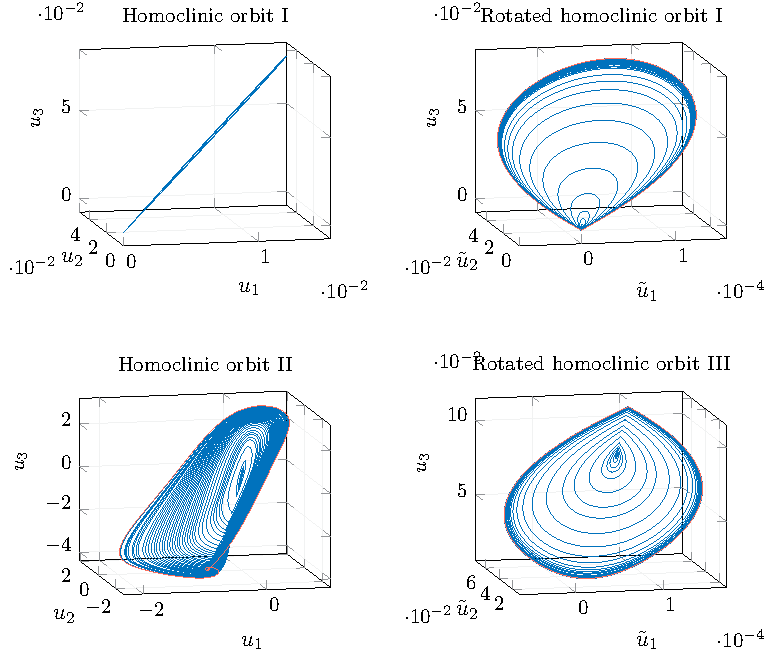
\includegraphics[width=\textwidth]{\imagedir/triNeuronBAMNeuralNetworkModelOrbitsPhaseSpace.pdf}
    \caption{
    Plots of homoclinic solutions emanating from the generic and transcritical
    Bogdanov--Takens bifurcations in \cref{sm:eq:tri_neuron_BAM-u}. In the top
    left plot the homoclinic solutions emanating from the transcritical
    Bogdanov--Takens point with fixed saddle points are shown. In the top right
    plot, we rotated the $(u_1, u_2)$ coordinates in order to make these
    homoclinic solutions visible. The bottom left plot shows the second branch
    of homoclinic solutions emanating from the transcritical Bogdanov--Takens
    point. Lastly, in the bottom right plot, the homoclinic solutions emanating
    from the generic Bogdanov--Takens point are shown. Here also the $(u_1,
    u_2)$ coordinates are rotated.
    }
    \label{sm:fig:triNeuronBAMNeuralNetworkModelOrbitsPhaseSpace}
\end{figure}


\subsection{Compare homoclinic solutions in phase-space}
Here, we compare the corrected and uncorrected profiles of the homoclinic
solutions on the two homoclinic curves emanating from the transcritical
Bogdanov--Takens point with the perturbation parameter ranging from $0.003$ to
$0.009$.
The code below produces (a figure similar to)
\cref{sm:fig:triNeuronBAMNeuralNetworkModelCompareOrbitsPhaseSpace}. We see
that the corrected and predicted homoclinic orbits are nearly identical.
\inputminted[firstline=356, lastline=385]{MATLAB}{\pathToDDEBifToolDemos/BAM_neural_network_model/BAMnn.m}
%
\begin{figure}[ht]
    \includetikzscaled{triNeuronBAMNeuralNetworkModelCompareOrbitsPhaseSpace}
    \caption{Plot comparing the third-order homoclinic asymptotics with the
        Newton correct homoclinic solutions in $(\epsilon,\tilde t, u_1)$
        phase-space. Here $\tilde t$ is the time $t$ rescaled to the interval
        $[0,1]$.
    }
    \label{sm:fig:triNeuronBAMNeuralNetworkModelCompareOrbitsPhaseSpace}
\end{figure}

\subsection{Continue periodic solutions from Hopf branch to homoclinic branch}
We continue a branch of periodic solutions emanating from point number 29 on the
first Hopf branch emanating from the transcritical Bogdanov--Takens point. The
periodic solution converges to a homoclinic orbit located on the second
homoclinic branch emanating from transcritical Bogdanov--Takens point. We will
use point number 28 on the periodic solution branch to compare against the
simulation in Julia in \cref{sm:sec:triNeuralBAMNetworkModelSimulation}. The
code below produces (a figure similar to)
\cref{sm:fig:triNeuronBAMNeuralNetworkModelPeriodicSolutions}.
\inputminted[firstline=387, lastline=391]{MATLAB}{\pathToDDEBifToolDemos/BAM_neural_network_model/BAMnn.m}
\vspace*{-12pt}
\inputminted[firstline=398, lastline=414]{MATLAB}{\pathToDDEBifToolDemos/BAM_neural_network_model/BAMnn.m}
\begin{figure}[ht]
    \includetikzscaled{triNeuronBAMNeuralNetworkModelPeriodicSolutions}
    \caption{
        Branch of periodic solutions emanating from the last point on the first
        Hopf branch emanating from the transcritical Bogdanov--Takens point in
        \cref{sm:eq:tri_neuron_BAM-u}. The last point on the perioidic solution
        branch is colored red, at which the periodic orbits have converged to
        a homoclinic orbit.
    }
    \label{sm:fig:triNeuronBAMNeuralNetworkModelPeriodicSolutions}
\end{figure}

\subsection{{\ifthesis \phantom{ } \fi} Homoclinic branch connecting the two Bogdanov--Takens {\ifthesis \phantom{ } \fi} points}
Here we will show that the transcritical and generic
Bogdanov--Takens points are connected, not only by a Hopf curve, but also
through a homoclinic curve. For this, we first continue the 
second Hopf branch emanating from the transcritical Bogdanov--Takens point again,
but with a smaller step size.
\inputminted[firstline=416, lastline=429]{MATLAB}{\pathToDDEBifToolDemos/BAM_neural_network_model/BAMnn.m}
%
Next, we continue from (almost) each point on the new Hopf branch the emerging periodic solutions in the parameter $\alpha_2$.
\inputminted[firstline=436, lastline=446]{MATLAB}{\pathToDDEBifToolDemos/BAM_neural_network_model/BAMnn.m}
%
By plotting the last point on each of the periodic solutions branches in
$(\alpha_1, \tilde u_1, \tilde u_2)$-space,
together with the homoclinic solutions on the first and third homoclinic branches continued
above, it is indeed clear that the two homoclinic branches are connected through a
single homoclinic curve, see
\cref{sm:fig:triNeuronBAMNeuralNetworkModelConnectionHomoclinicSolutions}.
We also see how the transition is made from the homoclinic orbits with a fixed saddle point
at the origin to the homoclinic orbits with a moving saddle. Clearly, \DDEBIFTOOL has
difficulties continuing the homoclinic orbits near the global homoclinic bifurcation point.
\inputminted[firstline=461, lastline=490]{MATLAB}{\pathToDDEBifToolDemos/BAM_neural_network_model/BAMnn.m}
%
\begin{figure}[ht]
    \includetikzscaled{triNeuronBAMNeuralNetworkModelConnectionHomoclinicSolutions}
    \caption{
        Branch of homoclinic solutions (orange) connecting the transcritical Bogdanov--Takens point (the right black dot) with
        the generic Bogdanov--Takens point (the left black dot) in
        \cref{sm:eq:tri_neuron_BAM-u}. The blue homoclinic curve emerging from 
        the transcritical and generic Bogdanov--Takens points are the previously continued
        homoclinic branches.
     }
    \label{sm:fig:triNeuronBAMNeuralNetworkModelConnectionHomoclinicSolutions}
\end{figure}
To obtain an impression of the parameter curves connecting the transcritical and
generic Bogdanov--Takens points, we rotated the  curves through an angle of $\theta_2=0.646045233034992$.
By doing so, the two Bogdanov--Takens points are aligned on the abscissa. In
\cref{sm:fig:triNeuronBAMNeuralNetworkModelConnectionHomoclinicParameters}, we plotted the first and third homoclinic branch, emanating from the
transcritical Bogdanov--Takens and generic Bogdanov--Takens points
respectively, the Hopf curve connecting the two Bogdanov--Takens points, and
the newly obtained homoclinic bifurcation curve.
\inputminted[firstline=501, lastline=529]{MATLAB}{\pathToDDEBifToolDemos/BAM_neural_network_model/BAMnn.m}
\begin{figure}[ht]
    \centering
    \includetikzscaled{triNeuronBAMNeuralNetworkModelConnectionHomoclinicParameters}
    \caption{
    Bifurcation diagram near the transcritical and generic Bogdanov--Takens
    bifurcation points in \cref{sm:eq:tri_neuron_BAM-u} showing the fully continued
    homoclinic branch connected to the non-trivial equilibrium emanating from the
    transcritical Bogdanov--Takens point.}
    \label{sm:fig:triNeuronBAMNeuralNetworkModelConnectionHomoclinicParameters}
\end{figure}


\subsection{Convergence plot}
\label{sm:sec:tri_neuron_BAM:convergence_plot}
Using the function from \cref{sm:lst:convergence_plot}, we create a log-log
convergence plot comparing the convergence order of the first and thrid order
homoclinic asymptotics from \cref{btdde:sec:transcritical_bt_homoclinic_asymptotics}.
The code below yields \cref{sm:fig:triNeuralBAMNetworkModelConvergencePlot}.
\inputminted[firstline=531, lastline=542]{MATLAB}{\pathToDDEBifToolDemos/BAM_neural_network_model/BAMnn.m}
\begin{figure}[ht]
    \centering
    \includetikz{triNeuralBAMNetworkModelConvergencePlot}
     \caption{On the abscissa is the approximation to the amplitude $A_0$ and on
        the ordinate the relative error $\delta$ between the constructed solution
        \mintinline{MATLAB}{hcli_pred} to the defining system for the homoclinic orbit
        and the Newton corrected solution \mintinline{MATLAB}{hcli_corrected}.}
    \label{sm:fig:triNeuralBAMNetworkModelConvergencePlot}
\end{figure}

\subsection{Simulation with {\tt DifferentialEquations.jl}}
\label{sm:sec:triNeuralBAMNetworkModelSimulation}
Here we will perform four simulations. The first two simulations will be at two
homoclinic orbits located on the two homoclinic curves emanating from the
transcritical Bogdanov--Takens point continued with \DDEBIFTOOL, see
\cref{sm:fig:triNeuralBAMNetworkSimulationHomoclinic}. The second two simulations will be in
the regions where there should be stable periodic orbits, see
\cref{sm:fig:triNeuralBAMNetworkSimulationPeriodic}.

\begin{figure}[ht]
    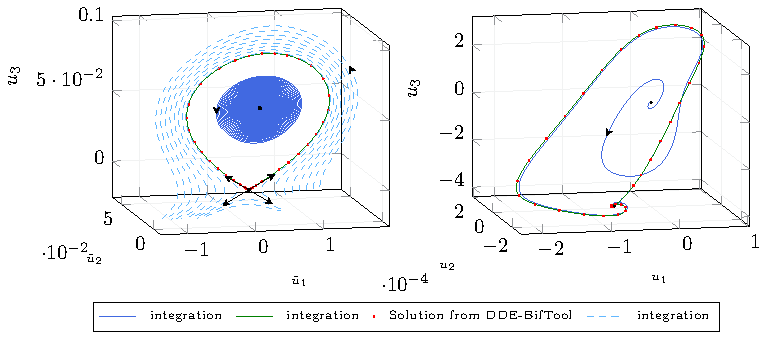
\includegraphics{\imagedir/triNeuralBAMNetworkModelHomoclinicSimulation.pdf}
    \caption{Comparing the computed homoclinic orbits in \cref{sm:eq:tri_neuron_BAM-u}
    with \DDEBIFTOOL with the solutions obtained from numerical simulation with Julia.
    We see the numerical integrated solution
    going through all the red points from the solution from \DDEBIFTOOL.}
    \label{sm:fig:triNeuralBAMNetworkSimulationHomoclinic}
\end{figure}

\begin{figure}[ht]
    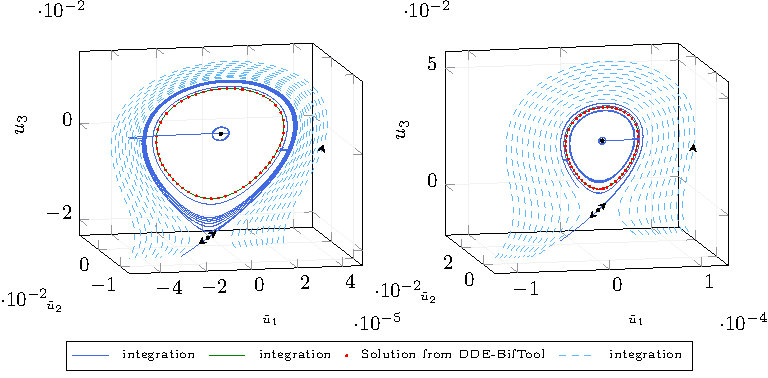
\includegraphics{\imagedir/triNeuralBAMNetworkModelPeriodicSimulation.pdf}
    \caption{Comparing the computed periodic orbits in \cref{sm:eq:tri_neuron_BAM-u}
    with \DDEBIFTOOL with the solutions obtained from numerical simulation with Julia.
    We see the numerical integrated solution
    going through all the red points from the solution from \DDEBIFTOOL.}
    \label{sm:fig:triNeuralBAMNetworkSimulationPeriodic}
\end{figure}

\subsubsection{Loading necessary Julia packages}
We start by loading the necessary Julia packages. Compared with the previous
demonstrations, we also need to load the Julia package {\tt Symbolics.jl} \cite{Symbolics.jl} to
differentiate the activation functions $f_1,f_2,f_3$.
\inputminted[firstline=1, lastline=9]{julia}{\pathToJuliaFiles/triNeuralBAMNetworkModel_simulation_article.jl}

\subsubsection{Define system}
Next we define the system to be integrated, a system to approximate the reverse
flow, and also an allocating version used for stability calculations. Note that
we need the Julia {\tt Symbolics.jl} to differentiate the activation functions.
\inputminted[firstline=11, lastline=63]{julia}{\pathToJuliaFiles/triNeuralBAMNetworkModel_simulation_article.jl}

\subsubsection{Function for creating streamlines plot}
To obtain an impression of the flow near transcritical Bogdanov--Takens point,
we create a streamlines function. This is particularly useful for seeing the
flow around the stable manifold of the saddle-note.
\inputminted[firstline=65, lastline=77]{julia}{\pathToJuliaFiles/triNeuralBAMNetworkModel_simulation_article.jl}

\subsubsection{Create figure with several axes}
We create a figure containing multiple axis in which we will plot 
the homoclinic, periodic orbits, and the left and right-hand sides
of \cref{sm:eq:triNeuralBAMNetworkModel:tan}.
\inputminted[firstline=79, lastline=89]{julia}{\pathToJuliaFiles/triNeuralBAMNetworkModel_simulation_article.jl}

\subsubsection{Define parameters, equilibria}
We define parameters located on the continued homoclinic branch with
\DDEBIFTOOL. Then calculate the equilibria points in \cref{sm:eq:tri_neuron_BAM}
near the transcritical Bogdanov--Takens point.
\inputminted[firstline=91, lastline=98]{julia}{\pathToJuliaFiles/triNeuralBAMNetworkModel_simulation_article.jl}

\subsubsection{Plot equilibria and homoclinic orbit}
By plotting the homoclinic orbit obtained with \DDEBIFTOOL located at parameter
values 
\[
    (\alpha_1, \alpha_2) = (-0.001724521613831, 0.001344362436730),
\]
we can compare with the numerical simulations. As in the analysis with
\DDEBIFTOOL, we rotate the coordinates of the solutions to visualize the
solutions in phase-space.
\inputminted[firstline=100, lastline=110]{julia}{\pathToJuliaFiles/triNeuralBAMNetworkModel_simulation_article.jl}

\subsubsection{Leading eigenvectors}
Next, we calculate and plot the leading eigenvectors of the characteristic matrix at the saddle-node bifurcation point.
\inputminted[firstline=112, lastline=135]{julia}{\pathToJuliaFiles/triNeuralBAMNetworkModel_simulation_article.jl}

\subsubsection{Define callback}
Since we are only interested in the flow near the equilibria points, we create a
continuous callback to ensure the orbits do not become too large.
\inputminted[firstline=137, lastline=140]{julia}{\pathToJuliaFiles/triNeuralBAMNetworkModel_simulation_article.jl}

\subsubsection{Integrate the system at homoclinic orbits I}
Now we define the problem to be integrated and choose the algorithm to be used.
Then we integrate the system for a range of initial history functions using the
function \mintinline{julia}{streamlines}. Next, we integrate the system near
the inner equilibrium, i.e., the equilibrium inside the homoclinic orbit. This
equilibria should be an unstable spiral. We show the first and last part
of the obtained solutions. We see that the last part of the integrated solutions
completely overlap the homoclinic solution obtained with \DDEBIFTOOL.
\inputminted[firstline=142, lastline=165]{julia}{\pathToJuliaFiles/triNeuralBAMNetworkModel_simulation_article.jl}

\subsubsection{Add arrows on solutions}
Lastly, we add arrows to the obtained solutions and redraw the equilibria.
\inputminted[firstline=167, lastline=178]{julia}{\pathToJuliaFiles/triNeuralBAMNetworkModel_simulation_article.jl}
We should now obtain an interactive figure similar to the left figure in
\cref{sm:fig:triNeuralBAMNetworkSimulationHomoclinic}.

\subsubsection{Simulation near stable periodic orbit I}
The code for numerical simulation near the second homoclinic orbit, see the
right plot in \cref{sm:fig:triNeuralBAMNetworkSimulationHomoclinic}, is not
included here.

To show by integration the existence of a stable periodic orbit, we first
located a periodic orbit in \DDEBIFTOOL. This can be done by continuing a
branch of periodic orbits emanating from a point on the continued Hopf curves.
Then we load the profiles of the periodic orbits into Julia. We perform two
simulations. For the first we integrate with a constant history function equal
to a point inside the periodic orbit. The second simulation starts from the
unstable eigenvector of the characteristic matrix calculated above.
\inputminted[firstline=237, lastline=328]{julia}{\pathToJuliaFiles/triNeuralBAMNetworkModel_simulation_article.jl}
After running the above code, we should obtain a similar plot as in
\cref{sm:fig:triNeuralBAMNetworkSimulationPeriodic}.

\subsubsection{Stability of the center manifold}
To confirm \cref{sm:lemma:triNeuralBAMNetworkModelEigenvalues} nummerically we
consider again
\cref{sm:eq:triNeuralBAMNetworkModelFunctions,sm:eq:triNeuralBAMNetworkModelFixedParameters}.
The code below plots the left and right-hand sides of
\cref{sm:eq:triNeuralBAMNetworkModel:tan}. We see in
\cref{sm:fig:triNeuralBAMNetworkStabilityDeterminingFunction} that there are
two points of intersection.
\inputminted[firstline=421, lastline=439]{julia}{\pathToJuliaFiles/triNeuralBAMNetworkModel_simulation_article.jl}
\begin{figure}[ht]
    \centering
    \includetikzscaled{triNeuralBAMNetworkModelStabilityDeterminingFunction}
    \caption{Plot of the left and right-hand sides of
    \cref{sm:eq:triNeuralBAMNetworkModel:tan}. Points of intersection are
    canditates for the center manifold to lose its stability.}
    \label{sm:fig:triNeuralBAMNetworkStabilityDeterminingFunction}
\end{figure}
Using the function \mintinline{julia}{roots} from the package {\tt IntervalRootFinding.jl}
we search for points of intersection. 
\inputminted[firstline=441, lastline=444]{julia}{\pathToJuliaFiles/triNeuralBAMNetworkModel_simulation_article.jl}
In the Julia output we obtain
\begin{minted}{shell-session}
7-element Vector{Root{Interval{Float64}}}:
 Root([13.2309, 13.231], :unique)
 Root([19.2374, 19.2375], :unique)
 Root([19.7337, 19.7338], :unknown)
 Root([6.00301, 6.00302], :unique)
 Root([8.33333, 8.33334], :unknown)
 Root([13.5353, 13.5354], :unknown)
 Root([5.75402, 5.75403], :unknown)
 Root([8.33333, 8.33334], :unknown)
\end{minted}
Note that, since there are multiple discontinuities, there are many unknown
solutions returned. We extract the unique solutions from the list of solutions
and test if these provide solutions to the characteristic equation.
\inputminted[firstline=446, lastline=457]{julia}{\pathToJuliaFiles/triNeuralBAMNetworkModel_simulation_article.jl}
In the Julia output we obtain
\begin{minted}{shell-session}
The centermanifold is locally attractive for 0 < τ < 13.230934887939895.
\end{minted}

\begin{figure}[ht]
    \centering
    \includetikzscaled{triNeuralBAMNetworkModelEigenvalues}
    \caption{Plot of the leading eigenvalues at the analytically derived
    transcritical Bogdanov--Takens point with $\tau = 13.230934887939895$
    and $\omega = \omega(\tau)$ from \cref{sm:eq:BAM_omega}. At this
    point there are four eigenvalues on the imaginary axis. For
    $\tau > 13.230934887939895$ the center manifold is locally unstable.}
    \label{sm:fig:triNeuralBAMNetworkModelEigenvalues}
\end{figure}
\subsubsection{Calculate and plot stability at Bogdanov--Takens point}
We fininsh this demonstration by confirming the stability
of the transcritical Bogdanov--Takens point at $\tau = 13.230934887939895$
obtained in the previous section. In \cref{sm:fig:triNeuralBAMNetworkModelEigenvalues}
we have plotted the eigenvalues. We indeed see that at $\tau = 13.230934887939895$
the center manifold looses stability. Lastly, we also varified in the code
below that the the eiganvalues with positive imaginary part on the imaginary axis
is approximatly equal to the expression for $\omega$ obtained in \cref{sm:eq:BAM_omega}. 
\inputminted[firstline=459, lastline=467]{julia}{\pathToJuliaFiles/triNeuralBAMNetworkModel_simulation_article.jl}

